% !TEX TS-program = xelatex
% !BIB program = bibtex
% !TEX encoding = UTF-8 Unicode

\documentclass[
  twoside,
  openright,
  degree    = master,               % degree = master | doctor
  language  = english,              % language = chinese | english
  fontset   = default,             % fontset = default | template | system | overleaf
  watermark = true,                 % watermark = true | false
  doi       = true,                 % doi = true | false
]{ntuthesis}

% !TeX root = ./main.tex

% --------------------------------------------------
% 資訊設定(Information Configs)
% --------------------------------------------------

\ntusetup{
  university*   = {National Taiwan University},
  university    = {國立臺灣大學},
  college       = {理學院},
  college*      = {College of Engineering},
  institute     = {地質科學系暨研究所},
  institute*    = {Institute of Geosciences},
  title         = {國立臺灣大學碩博士畢業論文模版},
  title*        = {National Taiwan University (NTU) \\ Thesis/Dissertation Template in \LaTeX},
  author        = {陳季晴},
  author*       = {Ji Ching Chen},
  ID            = {R09224122},
  advisor       = {譚諤},
  advisor*      = {Eh Tan},
  date          = {2022-05-01},         % 若註解掉,則預設為當天
  oral-date     = {2022-05-01},         % 若註解掉,則預設為當天
  DOI           = {10.5566/NTU2018XXXXX},
  keywords      = {LaTeX, 中文, 論文, 模板},
  keywords*     = {LaTeX, CJK, Thesis, Template},
}

% --------------------------------------------------
% 加載套件(Include Packages)
% --------------------------------------------------

\usepackage[sort&compress]{natbib}      % 參考文獻
\usepackage{amsmath, amsthm, amssymb}   % 數學環境
\usepackage{ulem, CJKulem}              % 下劃線、雙下劃線與波浪紋效果
\usepackage{booktabs}                   % 改善表格設置
\usepackage{multirow}                   % 合併儲存格
\usepackage{diagbox}                    % 插入表格反斜線
\usepackage{array}                      % 調整表格高度
\usepackage{longtable}                  % 支援跨頁長表格
\usepackage{paralist}                   % 列表環境


\usepackage{lipsum}                     % 英文亂字
\usepackage{zhlipsum}                   % 中文亂字

% --------------------------------------------------
% 套件設定(Packages Settings)
% --------------------------------------------------


\begin{document}

% 封面與口試審定
% Cover and Verification Letter
\makecover                          % 論文封面(Cover)
\makeverification                   % 口試委員審定書(Verification Letter)

% 致謝與論文摘要
% Acknowledgement and Abstract
% !TeX root = ../main.tex

\begin{acknowledgement}

謝謝所有走在科學革命上前端的人。
感謝哥白尼與加利略對日心說的貢獻。
感謝萊布尼茲串連了微分與積分。 
感謝牛頓所建立的古典力學。
感謝達爾文提出的演化論。
感謝普朗克與愛因斯坦解開古典物理的兩朵烏雲,拉開物理學上嶄新的一頁。
感謝波耳的量子力學。
感謝韋格納提出大陸漂移說。
感謝威爾遜、所有板塊構造學說的建構者。
最後再次感謝牛頓跟所有板塊構造學說的建構者,前者讓我們相信這個世界的知識是可以被數學所量化的,後者讓地球科學成為可量化的科學。

謝謝這些革命者創造了自然科學上理論與實驗的更多可能。
  

\end{acknowledgement}       % 致謝(Acknowledgement)
% !TeX root = ../main.tex

\begin{abstract}

平坦隱沒(flat slab subduction)是一種特殊的隱沒系統,其隱沒板塊在一固定深度內維持近乎水平狀態持續上百公里,與一般隱沒帶有所區別。
現今自然界中的平坦隱沒發生在科克斯隱沒帶的墨西哥區域以及納茲卡隱沒帶的秘魯與智利區域,其確切形成原因尚未釐清。
儘管兩個隱沒系統板塊幾何相似,然而兩處的平坦深度有顯著的不同,在科克斯隱沒帶,平坦深度與莫荷面相當,僅45公里,而納茲卡隱沒帶的平坦深度可達100公里。
墨西哥平坦隱沒上方有多個活火山存在,且隱沒系統脫水作用活躍,為弱耦合隱沒帶; 然而秘魯與智利平坦隱沒區域自全新世以來便沒有火山活動,該區域多次的大規模地震事件表明其為強耦合隱沒帶。
隱沒板塊的物理特性直接影響隱沒系統的重力力矩,在正常的隱沒帶中,隱沒板塊的密度在玄武岩相變成榴輝岩後急遽增加,地殼與地函顯著的密度差產生重力,形成隱沒系統穩定的驅動力。
過去的平坦隱沒數值模型研究多半使用降低隱沒系統驅動力的方式達成平坦隱沒,因此鮮少將榴輝岩相變加入數值模型中。
隱沒板塊上方地函楔(mantle wedge)的動水壓力(hydrodynamic pressure)降低會大幅增加隱沒系統的吸力力矩(suction torque)量值,倘若吸力力矩能超越重力力矩對隱沒系統施加的影響,可能是形成平坦隱沒的重要原因之一,然而由於影響動水壓力的因素難以掌控,平坦隱沒的發生原因與時機還是一個開放性問題。

本研究利用地球動力學二維數值模型FLAC (Fast Lagrangian Analysis of Continua)分別模擬科克斯隱沒帶與納茲卡隱沒帶的平坦隱沒。
利用參數化模擬部分熔融與岩漿庫的效應以實現隱沒系統中的岩漿作用,並用以討論墨西哥與智利兩種截然不同的岩漿作用特徵。
研究結果顯示智利平坦隱沒模型需要一個蛇紋岩化橄欖岩較少的地函楔環境。
狹窄的地函楔蛇紋岩化橄欖岩在聚合板塊交界處形成細窄的低黏滯度通道,導致隱沒板塊上下地函的壓力差增加,進而增加隱沒系統中的吸力力矩,形成平坦隱沒。

智利模型的平坦隱沒長度略少於實際長度,然而隱沒板塊平坦段深度與觀測結果相符合。
該模型在運行的時間段內皆有持續的部分熔融事件發生,然而由於模型的上覆板塊溫度較低,因此岩漿庫存在時間不長,導致該模型並沒有火山島弧的出現。
岩漿來源多為橄欖岩部分熔融,少數的隱沒沉積物有熔融跡象。
智利區域的岩漿組成份分析認為平坦隱沒上方火成岩具有埃達克岩(adakites)特徵,然而其形成機制確切原因還有待商榷。
墨西哥平坦隱沒模型則需要大量沉積物與蛇紋岩化橄欖岩的存在,且具備溫暖的上覆板塊與較快速的聚合速率。
該模型的平坦深度同樣吻合目前地震學觀測結果,平坦隱沒長度略少於實際長度。
模型中的部分熔融源在平坦隱沒生成之前為普通的橄欖岩,然而在平坦隱沒生成之後,決大部分熔融源皆為隱沒板塊上的沉積物與玄武岩物質,該結果與墨西哥平坦隱沒上方的埃達克岩紀錄相吻合。


\end{abstract}

\begin{abstract*}

Flat slab subduction, where the subducting slab moves sub-horizontally for hundreds of kilometres before diving into deeper mantle, is one of the most famous unusual subduction processes.
Flat slab subduction is recognised only in the Cocos and Nazca Plates in the present-day.
The reasons that the Cocos (Mexico) and Nazca (Chile and Peru) subduction zones develop from steep to flat subduction are not well understood.
While the geometry of the subducting plates is similar in these two regions, the flat slab depth is 45 km near the Moho in Cocos subduction zone and 100 km under lithosphere in Nazca subduction zone, respectively.
By the observation, Mexico flat slab subduction has a weak interface between the subducting plate and the upper plate, which leads to weak coupling.
Chile flat slab subduction generates a compression state on the upper plate, showing a strong coupling along the subducting plate.
The magmatism process is also different in Mexico and Chile.
While the volcano is still active above Cocos subdiction zone, the last active volcano above Nazca subduction occurred in the Miocene.
Adakites rocks are found in the far trench inland in both of these subduction zone.
There were many disputes over the formation mechanism between these two regions.

The purpose of this study is to explore flat slab subduction processes by using 2D thermo-mechanical models with Fast Lagrangian Analysis of Continua (FLAC) technology. 
We considered rock rheology of both elasto-plastic and visco-elastic deformations. 
To achieve the dehydration process during subduction, we parameterized the serpentinized peridotite by transforming the peridotite into a fixed thickness and realised the magma formation by tracking the P-T (pressure-temperature) path of markers.

Our results indicate the Chile flat subduction model requires a relatively small amount of serpentinized peridotites, which generates a thin low viscosity channel and a large pressure contrast between sub-slab mantle and mantle wedge, resulting in high suction force in the subduction system. 
The strong compression stress occurs in the top of the upper plate and subduction interface shows a strong coupling in the subduction system. 
Through the partial melting occurs continuously, the cold continental lithosphere leads to the fast decay of magma chamber. 
Therefore, the Chile flat slab model does not show any volcanic arc on the surface. 
By contrast, the Mexico flat slab subduction requires a warm overriding plate with high convergence rate and a large amount of serpentinite on the top of the slab. 
The upper plate does not undergo any compression or extension process in the model. 
The melting rocks in Mexico flat slab model change with time. 
The peridotite material is the predominant source of the magma chamber before the flat slab subduction develops.
Sediment and basalt start to melt once the flat slab occurs, implying the existence of adakites rocks. 
Our study suggests that the formation mechanism of flat slab subduction is different between Cocos and Nazca subduction zones.
    
\end{abstract*}              % 摘要(Abstract)

% 生成目錄與符號列表
% Contents of Tables and Denotation
\maketableofcontents                % 目錄(Table of Contents)
\makelistoffigures                  % 圖目錄(List of Figures)
\makelistoftables                   % 表目錄(List of Tables)
% !TeX root = ../main.tex

\begin{denotation}[3cm]


\item[$E$]{
  能量
}

\item[$m$]{
  質量
}

\item[$c$]{
  光速
}

\item[$K$]{
  bulk modulus
}

\item[$T$]{
  時間
}

\item[$v$]{
  速度
}

\item[$C_p$]{
  比熱
}


\end{denotation}
            % 符號列表(Denotation)

% 論文內容
% Contents of Thesis
\mainmatter
% !TeX root = ../main.tex

\chapter{Introduction}

\section{Background}

Geosynclinal theory was one of the famous theory in the geological studies history. It was believed that the earth's crust deformed with vertical motion in each geoloical zone while the Plate tectonic theory claimed that the earth's crust deformed with horizontal motion. In Geosynclinal theory, geological zone occurred weathering, magmatism and matamporphism process during geological time scale. Since 1960s, geophysics was revolutionized by the discovery of plate tectonics, that is, the plate tectonic theory had been proposed. The heat heterogeneous in earth's interior lead to gravitational instability, and therefore the earth's surface manifestations as plate tectonics (Jordan, 1978). The plate tectonic theory first defined the uppermost layers which is outside the upper thermal boundary layer --- lithosphere which consist with crust and part of mantle. Since lithosphere broken into many plate, horizontal motion dominate the Earth's surface with tectonic deformation processes  occur in plate boundary. The convergent boundaries represented by the trench and subduction zone where one of the plate destroyed. The divergent boundaries represented by the mid-ocean-ridge system where plate produced. The transform faults os a famous example of which plates move laterally relative to each other (The solid earth, 2005). 

In the convergent plate boundary, the thermal state of old lithosphere is relative colder than the ambient mantle, which lead to a denser condition. The cold region is enough to generate a gravitational instability in the subduction zone. Therefore, the heavy lithosphere develop the trench and sink into mantle which is so-called "slab".  The main changes which occur in the subducting plate are the shallow reaction of the oceanic crust to eclogite and the changes deeper in the mantle of olivine to a spinel structure and then to post-spinel structures. Phase changes result in increases in the density of the subducting slab. In the meantime, slab remains cold with gravitational instability. Thermal contraction provides the greatest contribution to the overall driving force. (The solid earth, 2005; Turcotte and Schubert, 2002). The geometry of slab varies considerably on Earth, with variations in slab dip angle and bending curvature (Schellart, 2020).

Flat subduction is a tricker circumstances of subduction geometry. In the flat subduction area, a part of the slab attains a horizontal orientation for several hundred kilometers below the overriding plate while the others part of the slab sinks into the mantle with a normal slab dip.



\section{Review of flat subduction numerical models}

目前造成平坦隱沒發生的機制眾說紛紜。南美洲區域平坦隱沒的發生區域與隱沒的中洋脊有幾何上的相關性,海洋地殼上中洋脊與海洋高原的存在可能會導致總體密度較低、浮力較大,因此過去曾經隱沒的中洋脊被認為是造成平坦隱沒的主要原因。

Hunen et al., 2002最早將模型加入增厚的海洋地殼,以模擬過去智利與秘魯曾經有中洋脊與海洋高原進入隱沒帶中的紀錄。增厚海洋地殼有較低的密度與較大的浮力,其上方岩相需要比原先更大的壓力與更高的溫度才會從玄武岩相變成密度高的榴輝岩,可能使隱沒板塊與周遭地幔沒有顯著密度差而發生平坦隱沒。不過由於該研究模型僅二維,單純加入增厚海洋地殼所呈現的模型雖然能呈現平坦隱沒,但結果是假設第三維上有無限延伸的增厚海洋地殼,現實中增厚的海洋地殼能造成的浮力效應應遠小於二維模型中的結果。Florez-Rodr´ıguez et al., 2019在三維模型中證明了這一點,他們提出若將現在自然界中最大的洋脊隱沒進入地幔,其所提供的浮力也只會造成海洋板塊傾角減少原先的10度。若從自然界中來看,確實有許多區域皆有海脊隱沒的證據,例如勘察加半島(Kamchatka)有皇帝海脊(Emperor Ridge)隱沒、琉球(Ryukyu)有大東海脊(Daito Ridge)隱沒以及馬里亞納(Mariana)與馬庫斯—內克海脊(Marcus-Necker Ridge)隱沒,然而只有秘魯與智利有平坦隱沒的特徵。此外,在墨西哥有平坦隱沒的特徵,然而墨西哥沒有任何海脊或海洋高原的隱沒紀錄,因此增厚的海洋地殼發生平坦隱沒的理論近年來逐漸站不住腳(Schellart, 2020)。

Hunen et al., 2000 使用二維笛卡爾座標數值模型進行祕魯與智利平坦隱沒的模擬。在他們得模型中,唯一能成功演化出平坦隱沒的機制只有海溝後撤迫使大陸岩石圈逆衝到隱沒板塊之上。Liu and Currie, 2016 使用二維模型模擬過去股法拉隆板塊板塊的平坦隱沒機制,他們加入增厚的海洋地殼後並無法觸發平坦隱沒的產生,然而,再加入額外大陸岩石圈的水平速度後,平坦隱沒便能成功再現。Axen et al., 2018使用同樣的數值模型將古代北美西部的克拉通放置於大陸板塊測,成功模擬出增厚海洋地殼加上快速移動大陸岩石圈能發生平坦隱沒,並且能將克拉通從大陸岩石圈底部刮除,證實了平坦隱沒能破壞大陸岩石圈。在該研究中並沒有考慮克拉通對平坦隱沒的影響。

Manea et al., 2012提出了另外的看法。他們利用三維模型模擬過去30Ma以來智利區域的隱沒帶動態行為,使用額外施加的邊界條件強迫智利海溝後撤,發現海溝後撤能夠施加給隱沒板塊的地幔流吸力(suction)不足以讓巨大厚重的海洋板塊變平坦,因此他們在模型上覆板塊加上克拉通,系統性測試從150-300公里厚的大陸岩石圈與海溝距離600-1000公里時隱沒帶下方地幔流產生的動力壓力(dynamic pressure)。他們發現在只有在克拉通與海溝距離約800公里且克拉通厚度大於200公里時平坦隱沒才會生成。當他們把造成海溝後撤的邊界力移除時,不會觸發平坦隱沒的形成,因此他們得出的結論是需要同時有海溝後撤與克拉通的存在才會觸發平坦隱沒。這是首次將克拉通加進數值模型裡的平坦隱沒模型。隨後Liu and Currie, 2016效仿同樣的機制,將過去普遍認為存在於北美板塊西部下方的科羅拉多高原山根放入模型中,模擬古法拉龍板塊平坦隱沒演化。他們認為克拉通與山根的存在只是加快平坦隱沒的形成,但真正觸發平坦隱沒的機制是增厚海洋地殼延緩玄武岩相變成榴輝岩。Hu et al., 2016使用三維模型CitcomS模擬整個南美洲海溝45 Ma以來隱沒帶演化。在加入克拉通的模型中,隱沒板塊傾角有降低的趨勢,不過根據模型結果,真正造成平坦隱沒的形成依然與隱沒海脊相關,只有在海脊進入三維模型後隱沒傾角才出現顯著降低。

因此,目前的平坦隱沒數值模型大多以擬合智利、祕魯與法拉龍板塊為主,觸發平坦隱沒的機制大多與克拉通的存在與否、是否有洋脊隱沒以及上覆板塊的移動速度為主要測試,墨西哥區域尚未有平坦隱沒的數值模型被提出。在墨西哥,隱沒板塊上沒有任何增厚的紀錄,此外該地區北美板塊移動速率遠低於南美洲與過去法拉龍板塊隱沒時期的北美板塊,因此墨西哥區域的平坦隱沒機制尚未有統一定論。本研究期待能利用數值模擬得到墨西哥平坦隱沒從過去50 Ma以來的演化,並提出新的演化機制模型,填補過去尚未成熟的平坦隱沒機制理論。


\section{Motivation}

\section{Geophysical observation in Cocos subduction zone}

\section{Summery}

% !TeX root = ../main.tex

\chapter{Numerical modelling method}

The numerical models in this study address the dynamics process of flat subduction, in which an oceanic plate subducts beneath continental plate. The goal of this work is to address the controls on subducting plate dynamics and to determine the conditions under which flat subduction may develop. 

In this chapter, we introduce the method of numerical model and the initial model setup. In section 2.1, we discuss the governing equations. In section 2.2, the finite elements method will be briefly discuss. In section 2.3, we introduce the Fast Lagrangian Analysis of Continua technique. In section 2.4, the model geometry is presented. The material properties, phase transition and model boundary conditions are given in section 2.5 ,2.6 and 2.7, respectively.

\section{Governing equation}

\subsection{Continuum---Conservation of mass}

In geodynamics modelling, we consider major rock units as continuous geological media. The continuous description is described by field variables such as density, pressure, velocity, strain, etc. Since on long timescales geological unit behave like slowly creep fluids, geodynamics process in the viscous part (mantle) are often referred to as process of geodynamical fluid dynamics. 

The mass conservation equation in Lagrangian form is as follow
\begin{align}
\frac{\partial \sigma_{ij}}{\partial x_j}+\rho g_i = \rho \frac{\partial D_{vi}}{\partial t} 
\end{align}
The proof of eq.(2.1) is as follow
\begin{figure*}[ht!]
    \centering
    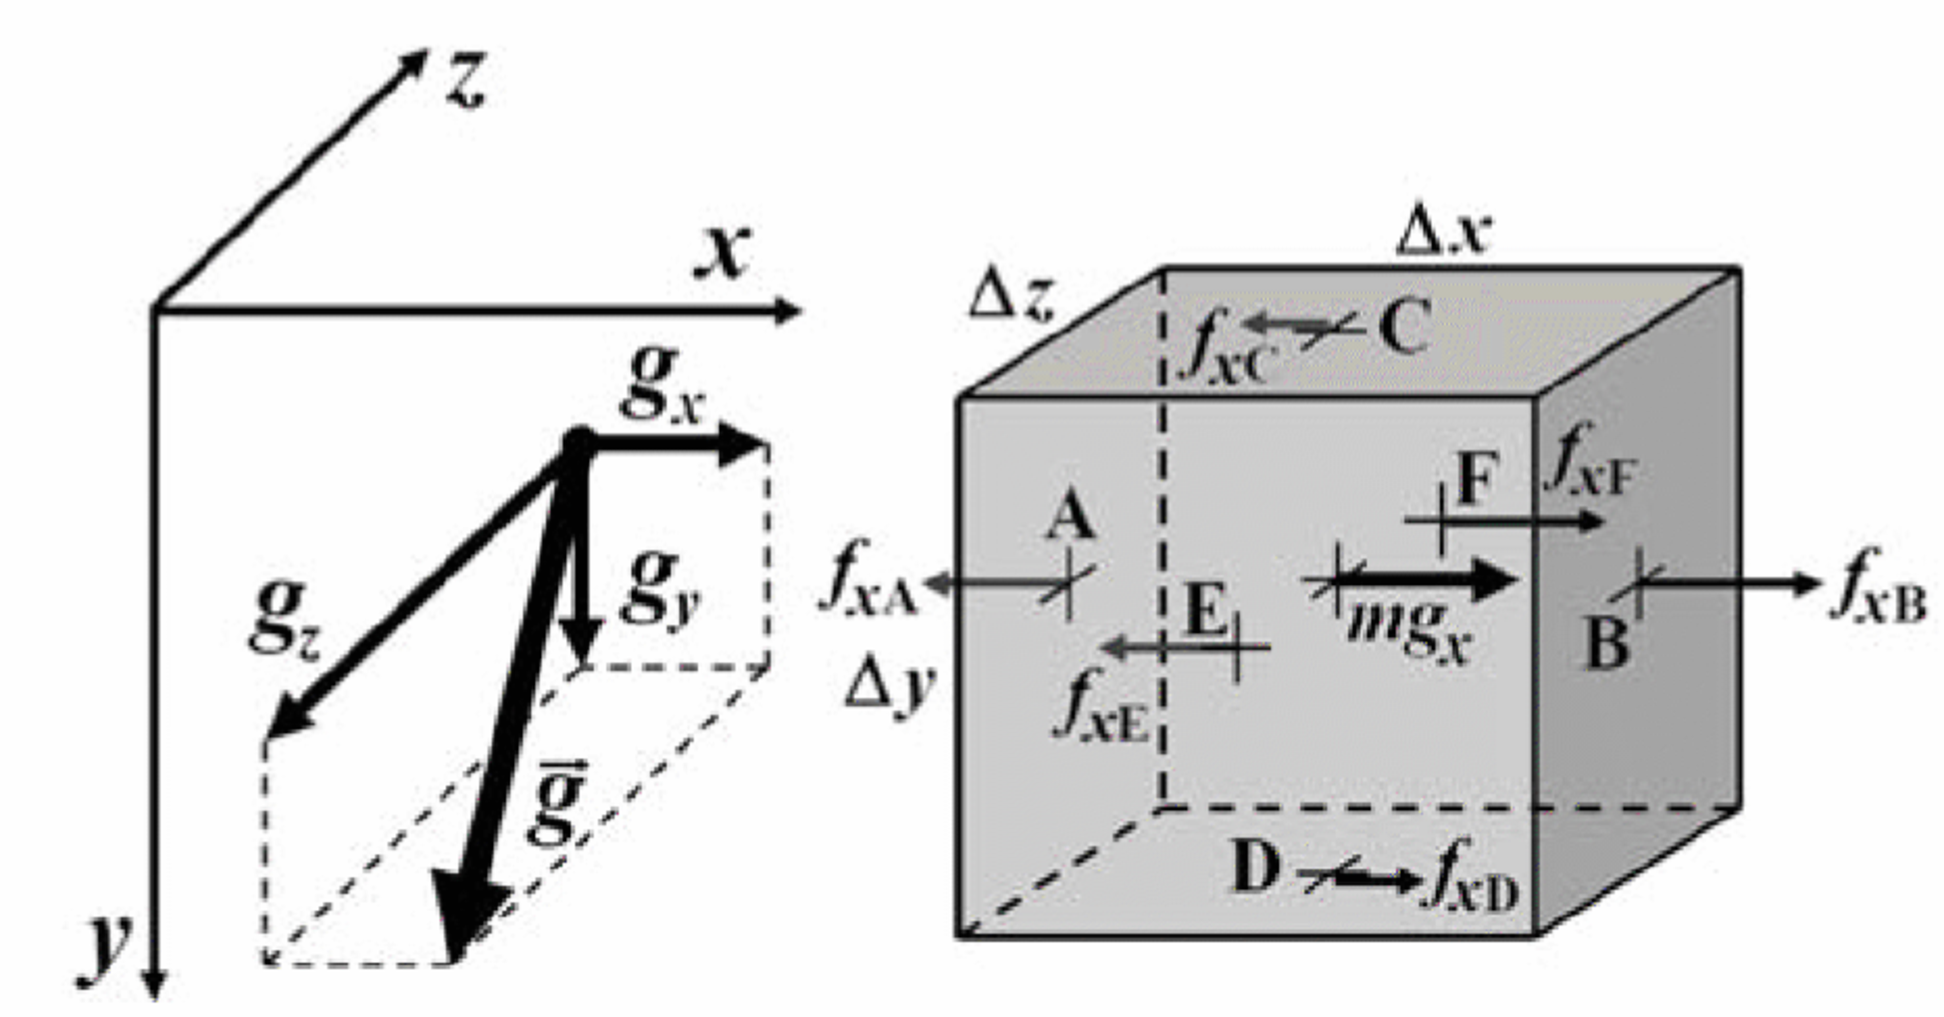
\includegraphics[width=4in]{momentum.pdf}
    \caption{ Model. }
    \label{fig::model}
\end{figure*}

There are totally two unknow: density and velocity.
While in geodynamics modelling, the density variations are small enough to be ignored, which is the result of Boussinesq approximation. The Boussinesq approximation assume that the density is linear proportional to the temperature and the small density variation is then neglected, except the gravity term.
\begin{align}
\rho (T) = \rho_0[1-\alpha (T-T_0)] 
\end{align}
where $\rho_0$ is the reference density at temperature $T_0$ and $\alpha$ is the volumetric thermal expansion coefficient. The boussinesq approximation also represent the incompressible condition, which mean the density of material points does no change with time. The incompressible continuity equation is broadly used in numerical geodynamic modelling, although on many cases it is rather big simplification. 
\begin{align}
\nabla \cdot (\vec v) = 0 
\end{align}
Eq. (2.3) is the conservation of mass in our numerical modelling approach.

\subsection{Motion---Conservation of momentum}
In geodynamics, the time-dependent phenomena involve deformation of continuous media, which is the effect of the balance of internal and external forces that act in these media. So as to relate forces and deformation, an equation of motion may be used --The momentum equation. The momentum equation is a differential equivalent of Newton’s second law to a continuous medium.

$f=ma$

Eulerian Form: $\frac{\partial \sigma_{ij}}{\partial x_j}+\rho g_i = \rho (\frac{\partial v_i}{\partial t}+v_j\frac{\partial v_i}{\partial x_j})$

Lagrangian Form: $\frac{\partial \sigma_{ij}}{\partial x_j}+\rho g_i = \rho \frac{\partial D_{vi}}{\partial t}$

F is the net force acting on the object which can be computed locally. 
We will proof the momentum equation of Lagrangian Form below:

For x-component
\begin{align}
f_x=f_{xA}+f_{xB}+f_{xC}+f_{xD}+f_{xE}+f_{xF}+mg_x 
\end{align}
$f_{xA}- f_{xF}$ are stress-related forces, from the outside of the volume on the resoective boundaries A-F. 
$f_g=m_gx$ is the gravity force.
\begin{align}
f_{xA} = -\sigma_{xxA}\Delta y\Delta z
\end{align}
\subsection{Heat equation --- Conservation of energy}

To describe the balance of energy in a continuum material, heat equation is apply to measure the temperature change. The heat equation sloved the heat transport and porvided the temperature field. Below is the heat equation in Lagrangian form :
\begin{align}
\rho C_p \frac{DT}{Dt} = -\frac{\partial q_x}{\partial x}-\frac{\partial q_y}{\partial y}-\frac{\partial q_z}{\partial z}+H_s+H_L
\end{align}

where $\rho$ is the density, $C_p$ is the heat capacity at constant pressure (isobaric heat capacity), $H_s$ is shear heating and $H_L$ is the latent heat production.

The proof of heat equation is show below:

(加上heat equation的推倒
加圖)


Base on the Boussinesq approximation, the imcompressible Lagrangian form governing equations are:

\begin{align}
\nabla \cdot (\vec v) = 0 
\frac{\partial \sigma_{ij}}{\partial x_j}+\rho g_i = \rho \frac{\partial D_{vi}}{\partial t}
\rho C_p \frac{DT}{Dt} = -\frac{\partial q_x}{\partial x}-\frac{\partial q_y}{\partial y}-\frac{\partial q_z}{\partial z}+H_s+H_L
\end{align}

Decribe conservation of mass, conservation of momentum and conservation of energy, respectively.


\section{Finite elements method}

finite elements method

\section{FLAC}

what is FLAC

We used the Fast Lagrangian Analysis of Continua (FLAC) technique.

\section{Initial Model}

initial model

\section{Rheological behavior}

**What is viscous and the viscous rheology of rock**

In the near-surface region, rocks undergo relatively low temperature and, therefore, the Earth's lithosphere easily result in brittle (at low pressure) and plastic (at high pressure) deformation. 
While in the deep earth, temperature increasing with depth, rocks behave viscous with irreversible deformation. 
Therefore, if a geodynamics model need to account for a wide range of rocks properties, it should consider the elasto-visco-plastic rheology of rocks.

\section{Phase change}

In this study, we use markers to trace the rocks phases, pressure and temperature. 
At the time the pressure and temperature satisfy the phase transformation condition, the marker will turns to new rock phase. 
A basalt element represent an element with more than 30 presents of the basalt phase markers. 
In this case, the element behave the deformation as same as the basalt rheology.

\subsection{Peridotite --- Serpentinite}

Once the subducting plate sink into mantle, sediment on oceanic plate undergo higher pressure and temperature that release a large amount of fluids. 
On the other hand, the oceanic plate itself also carries seawater into the mantle. 
Fluids in subduction zone mostly concentrated in the mantle wedge. 
The dry mantle wedge undergo hydration process, lead to the transformation of peridotite to serpentinite.  
The serpentinite depth and thickness in subduction zone is not well understand since the seismic study constrain still contain high uncertainly, we model the phase transformation process of serpentinite in parameter way.     

Serpentinite are stable in the colder mantle wedge relative to deeper mantle, and therefore once the serpentinite under unstable field, we assume that serpentinite rocks release fluid and transfer to peridotite. 
The following equations are the conditional expressions of serpentinite---peridotite transformation. Figure is the phase diagram of mantle phases.


\subsection{Basalt --- Eclogite}

As the oceanic crust sink into deeper mantle, the mafic rocks enters the eclogite stability field in the condition of high pressure. 
Therefore, basalt phases transform to eclogite.  
In this model, oceanic crust are tracked and compared with the eclogite stability filed, the following equations are the conditional expressions of mafic rocks transformation. 
Figure below is the mafic rocks phase diagram.

\subsection{Sediment --- Schist}

Once sediment undergo higher pressure, the compression process and mataphase(變質作用)process occur.
In this model, the following equations are the conditional expressions of transformation process of sediment to schist.

$T > 650^{\circ} C$\\
$depth >  20 $km 

The subducted sediments will turn into schist when temperature is greater than 650$^\circ$C and pressure is greater than (一個數字 算出來?)

\subsection{Hydrated olivine --- Peridotite}

We considering a hydrated peridotite under the oceanic crust in our model. 
The magma will only generated above the hydrated subducting oceanic lithosphere.
Once the tempertaure is too high to make the rock contain water, the hydrated olivine transform to normal perodotite.
The following equation is the conditional expression of this transgformation.

$T > 800-35\times 10^{-9}\times (depth-62)^{2\circ}C$

\section{Boundary condition}

\subsection{Kinematic boundary condition}

\subsection{Thermal boundary condition}

For oceanic lithosphere, we used half space cooling model in our model to defined the thermal condition. 
The plate depth is proportional to the square root of oceanic lithosphere age, and therefore, the half space cooling model can predict will for the temperature of the oceanic plate.
Follow by David and Lister,1974:

$T=T_m\cdot {erf}(\frac{z}{2\sqrt{\kappa t}})$

$T$ is the temperature, $T_m$ is the mantle temperature, in this model the temperature is 1330,
$z$ is the depth from surface and $\kappa$ is the thermal conductivity ceoficient, that is, $10^{-6}$ in this study.
$t$ is the lithosphere age in Myr.


For continental lithosphere, the thermal condition is defined in linearly.



% !TeX root = ../main.tex

\chapter{數值模型結果}

\section{智利參考模型}
\subsection{初始模型設定}
本研究建立一個長1200公里、深300公里的長方形二維剖面,包含一段長425公里的海洋岩石圈與775公里的大陸板塊,在兩個板塊交界處,建立一段長度31公里傾角35度的隱沒板塊,交接處區域的溫度較高,方便隱沒帶發育。
智利參考模型設計見圖\ref{fig::reference Nazca model}。
海洋岩石圈年齡為40個百萬年(\citealp{muller2019}),包含2公里厚的沉積物、6公里厚的玄武岩與10公里厚的綠泥岩,其熱構造由第二章式\ref{eq:Half Space Model}提及的半空間冷卻模型決定。

\begin{figure*}[hb]
    \centering
    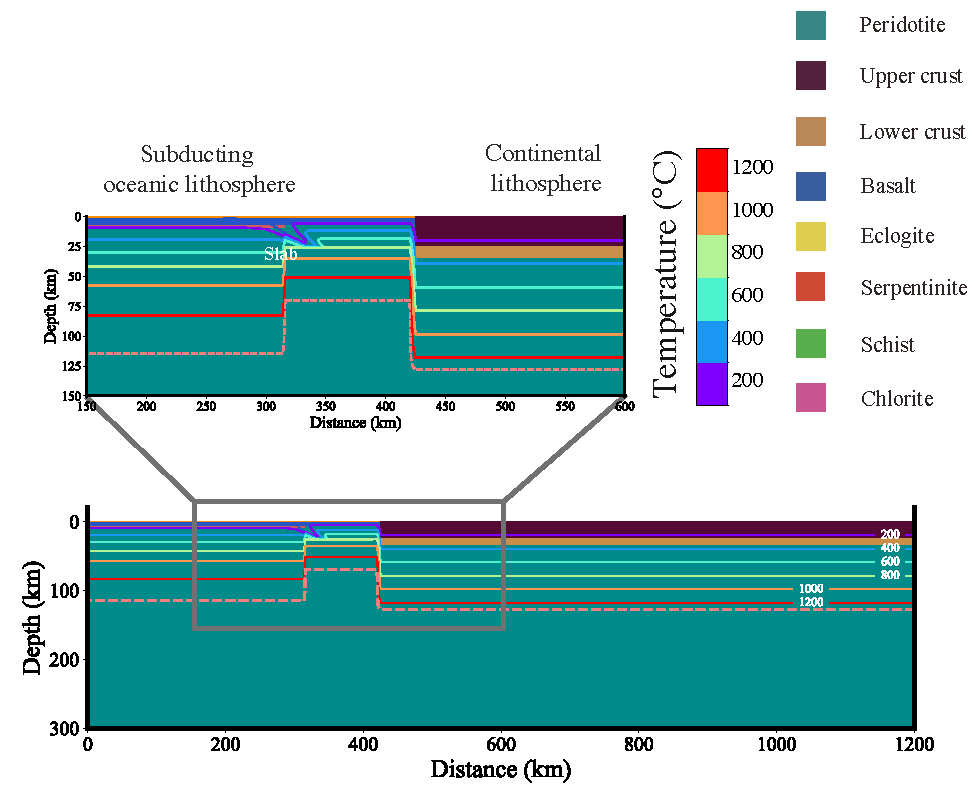
\includegraphics[width=6in]{Ref_Nazca.pdf}
    \caption[智利參考模型設計與邊界條件示意圖]{智利參考模型設計與邊界條件示意圖}
    \label{fig::reference Nazca model}
\end{figure*}

大陸岩石圈包含25公里厚的上部地殼(upper crust)與10公里厚的下部地殼(lower crust),由於秘魯與智利平坦隱沒區域的大陸地溫梯度資料較少,過去研究並沒有很好的約束,僅透過重力資料推測彈性岩石圈厚度大約140公里,因此模型設定地溫梯度以每公里攝氏9.5$^{\circ}$線性遞增至140公里深(\citealp{perez2008})至岩石圈底部1330$^{\circ}$。
地表溫度皆為攝氏10$^{\circ}$,模型底部溫度固定攝氏1330$^{\circ}$。

由於現生地震學觀測研究提及該地區地震活動度大,且地函岩石圈速度較高、板塊脫水作用不活躍,因此智利參考模型的蛇紋岩厚度參數設定為5公里。模型左邊界從地表至300公里深皆以等速率每年6公分往右移動,右邊界則固定不動。
本研究速度參考來自於\citealp{o2005uncertainties},使用印度-大西洋熱點參考座標(Indo-Atlantic hotspot reference frame)中的相對板塊運動模型計算(\citealp{schellart2008global})。

模型上邊界為自由表面,而下邊界則為開放邊界,物質可自由進出。
需要注意現今的秘魯與智利平坦隱沒區皆落在安地斯山脈造山範圍,然而本參考模型沒有包含造山運動。
就現今觀測資料來看,平坦隱沒事件早於安地斯造山事件(\citealp{chen2019southward}; \citealp{hu2021southward}),兩者並沒有直接關係。


\subsection{智利參考模型結果}\label{智利參考模型結果}
智利參考模型產生一深度約100-110公里、長度約300公里的平坦段。

在隱沒初始時期,隱沒作用促使地函流上湧,導致地函楔溫度升高,同時強烈的岩石變形與破壞導致隱沒板塊交界處產生摩擦熱,海洋地殼溫度被動上升。
岩石在一系列的加溫下發生相變,隱沒地殼上的玄武岩相在約攝氏500$^{\circ}$等溫線(深度40公里處)處相變成緻密的榴輝岩相,如圖\ref{fig::Nazca_Ref_26}a所示。
榴輝岩相密度遠大於周遭地函密度,顯著的密度差造成隱沒系統中的重力不穩定,促使隱沒板塊驅動力產生,隱沒系統得以順利發育,隱沒帶密度剖面見圖\ref{fig::Nazca_Ref_26}c。

海洋地殼上的沉積物在隱沒過程中絕大比例在海溝處堆積,形成厚度約10公里的增積岩體,僅有少部分沉積物被帶入地函中,這些沉積物與海水隨著地殼進入高溫高壓環境。
離開近地表後,地殼上的黏土礦物逐漸進入不穩定狀態,釋放出晶格中的水分,導致地函楔中的橄欖岩發生水合作用(hydration reaction)而相變成蛇紋岩化的橄欖岩(serpentinized peridotite),其與隱沒的沉積物一同在地函楔中形成強度低且密度較低的低黏滯度通道(low viscosity channel),見圖\ref{fig::Nazca_Ref_26}b與圖\ref{fig::Nazca_Ref_51}b模型黏滯度剖面。

在地函較深處,蛇紋岩化的橄欖岩進入更高溫的環境發生脫水,於深度70公里處相變回橄欖岩。
由於70公里深的環境已達到攝氏700$^{\circ}$,岩石幾乎都以黏性變形為主,因此低黏滯度通道在蛇紋岩化橄欖岩脫水後依然存在於板塊交界處中。

海洋板塊中的綠泥岩在120-130公里深處發生脫水,相變成普通的橄欖岩。
儘管綠泥岩脫水作用導致地函楔中的熔點下降,然而隱沒早期板塊溫度較低,即便進入地函楔中依然難以達到岩石熔點。

隱沒早期強烈的聚合作用在大陸岩石圈攝氏600$^{\circ}$等溫線之上方產生一厚度25公里、寬度150公里的高壓帶,詳見圖\ref{fig::Nazca_Ref_26}d動態壓力剖面紅色區域。
該高壓帶在10 Myr便不復存在,隨著隱沒持續進行,低黏滯度通道的存在隔絕上覆板塊、隱沒板塊與地函楔之間的物質交換,地函流
地函楔頂部、板塊交界處壓力降低,於80-120公里深處形成低壓區,見圖\ref{fig::Nazca_Ref_51}d深藍色區域。 
低壓區域促使動水壓力力矩增加,超過重力力矩,在模型隱沒系統中形成一逆時針方向上的轉動,直接促使隱沒板塊傾角(dip)快速降低(見圖\ref{fig::Nazca_Ref_slab_time})。

隨著隱沒板塊傾角降低,其下方因承受強烈彎曲(bending),在模型時間10-15 Myr之間於地函楔低壓區下方、隱沒地函岩石圈(subducting mantle lithosphere)處形成另一寬度約100公里的高壓區,見圖\ref{fig::Nazca_Ref_76}d紅色區域。
隱沒板塊下方的高壓帶與隱沒板塊上方的低壓帶平行於隱沒板塊,在隱沒板塊上
產生壓力梯度力,該力垂直作用於隱沒板塊。
在轉動系統中,壓力梯度力造成該隱沒段於逆時針方向上的力矩急遽增大,見圖\ref{fig::Nazca_Ref_torque_time},因此在模型時間15 Myr後形成平坦隱沒。

這段時間內因隱沒傾角漸緩,地函楔橄欖岩在壓力不變的情形下溫度逐漸上升,有部分岩石通過固相線,發生些許部分熔融事件,部分熔融位置於圖\ref{fig::Nazca_Ref_76}c中黃線處,部分熔融比例見圖\ref{fig::Nazca_Ref_melting_time}(a)。

隨後模型至30 Myr,平坦隱沒持續發育,其深度大致與原先大陸岩石圈攝氏800$^{\circ}$等溫線深度相同,在模型中約略100-120公里深(圖\ref{fig::Nazca_Ref_76}a、\ref{fig::Nazca_Ref_101}a、\ref{fig::Nazca_Ref_126}a、\ref{fig::Nazca_Ref_150}a)。
隱沒板塊在達到攝氏900$^{\circ}$等溫線前後離開平坦段,在深度120公里之後形成一高角度隱沒板塊。

因低黏滯度通道狹窄,隔絕地函流進入地函楔中,因此隱沒板塊上方的黏滯度持續維持低壓狀態。
此外,平坦隱沒上凹區域因強烈彎曲形成高壓帶,與板塊上方地函低壓帶形成的壓力梯度同樣垂直於隱沒板塊,因此在20 Myr之後,與重力力矩相比,動水壓力力矩維持穩定優勢,隱沒板塊與上覆板塊被牢牢吸住(圖\ref{fig::Nazca_Ref_76}b, d、\ref{fig::Nazca_Ref_101}b, d、\ref{fig::Nazca_Ref_126}b, d、\ref{fig::Nazca_Ref_150}b, d)。


\begin{figure*}[htp]
    \centering
    \includegraphics[width=6in]{Ref_Nazcaframe_26_snapshot_5field_200_v1.pdf}
    \caption[智利參考模型於5 Myr時之結果。]{智利參考模型於5 Myr時之結果。}
    \label{fig::Nazca_Ref_26}
\end{figure*}

\begin{figure*}[htp]
    \centering
    \includegraphics[width=6in]{Ref_Nazcaframe_51_snapshot_5field_200_v1.pdf}
    \caption[智利參考模型於10 Myr時之結果。]{智利參考模型於10 Myr時之結果。}
    \label{fig::Nazca_Ref_51}
\end{figure*}

\begin{figure*}[htp]
    \centering
    \includegraphics[width=6in]{Ref_Nazcaframe_76_snapshot_5field_200_v1.pdf}
    \caption[智利參考模型於15 Myr時之結果。]{智利參考模型於15 Myr時之結果。}
    \label{fig::Nazca_Ref_76}
\end{figure*}

\begin{figure*}[htp]
    \centering
    \includegraphics[width=6in]{Ref_Nazcaframe_101_snapshot_5field_200_v1.pdf}
    \caption[智利參考模型於20 Myr時之結果。]{智利參考模型於20 Myr時之結果。}
    \label{fig::Nazca_Ref_101}
\end{figure*}

\begin{figure*}[htp]
    \centering
    \includegraphics[width=6in]{Ref_Nazcaframe_126_snapshot_5field_200_v1.pdf}
    \caption[智利參考模型於25 Myr時之結果。]{智利參考模型於25 Myr時之結果。}
    \label{fig::Nazca_Ref_126}
\end{figure*}


\begin{figure*}[htp]
    \centering
    \includegraphics[width=6in]{Ref_Nazcaframe_150_snapshot_5field_200_v1.pdf}
    \caption[智利參考模型於30 Myr時之結果。]{智利參考模型於30 Myr時之結果。}
    \label{fig::Nazca_Ref_150}
\end{figure*}
\newpage
\subsection{模型脫水位置與岩漿作用}
上述的剖面無法精確看到島弧位置,因為整個隱沒系統產生的島弧量非常少。
模型中發生部分熔融與海溝之距離隨時間變化如圖\ref{fig::Nazca_Ref_melting_time}a所示。
普通的隱沒帶火山島弧與海溝的距離絕大部分落在100公里左右(\citealp{peacock1990fluid}; \citealp{hyndman2003serpentinization}),然而在智利參考模型中,平坦隱沒的生成促使岩漿作用位置遠離海溝,並且隨著時間逐漸往內陸移動,最大可達近500公里。
除此之外,圖\ref{fig::Nazca_Ref_melting_time}a暗示著島弧往內陸移動速率變化,在25 Myr之前的島弧移動速率快速,斜率較大,然而在平坦隱沒發育後,島弧移動速率趨近緩和,斜率較小。


\begin{figure*}[hb]
    \centering
    \includegraphics[width=4in]{Ref_Nazca_melting_time_v1.pdf}
    \caption[智利參考模型岩漿作用隨時間變化]{智利參考模型岩漿作用隨時間變化,灰色底標出平坦隱沒發育後時間段。(a)部分熔融與海溝之距離隨時間變化圖,縱軸中每個點代表每次部分熔融發生位置,顏色為指數上的部分熔融比例。(b)岩石熔融量隨時間變化圖,熔融量單位為每單位海溝產生之立方公里量中每20萬年瞬時量。顏色代表不同岩相。}
    \label{fig::Nazca_Ref_melting_time}
\end{figure*}

部分熔融量隨時間變化如圖\ref{fig::Nazca_Ref_melting_time}b。
在平坦隱沒發育穩定後,隱沒板塊進入大陸岩石圈內側,不斷降低地函楔溫度。
因此在平坦隱沒形成後5個百萬年之內,岩石熔融量快速減少,至30 Myr後每20萬年僅有不到1立方公里岩石熔融。
圖中顯示岩漿作用活躍度在20 Myr前後達到高峰,並且在平坦隱沒發育後有些微沉積物熔融的現象,最終在45 Myr前後不再有部分熔融事件發生,進入岩漿停止期,此現象與該地區的岩漿觀測資料吻合。

將模型中部分熔融事件與岩漿庫絕對位置繪出,分別獲得圖\ref{fig::Nazca_Ref_2Dtime_series}a, 圖\ref{fig::Nazca_Ref_2Dtime_series}b。
在模型中10-25 Myr時,部分熔融與岩漿庫快速往內陸移動,隨後在30-50 Myr後部分熔融事件與岩漿庫位置維持穩定,表示模型已達動態平衡。

玄武岩至榴輝岩相變位置見圖\ref{fig::Nazca_Ref_2Dtime_series}c。
玄武岩相變位置在早期約50公里深,而直到30 Myr來到80公里深,並且有逐漸遠離海溝的趨勢。
由於隱沒系統持續穩定隱沒,導致大陸岩石圈近海溝側溫度逐漸變冷,因此玄武岩相變也往更深且更內陸的方向移動,最終在約80公里深,模型絕對座標450-460公里左右收斂。
儘管該結果顯示玄武岩相變位置逐漸往更深更遠離海溝,導致在300公里深範圍內的隱沒板塊重力力矩可能會些許減少。然而,由圖\ref{fig::Nazca_Ref_time}b平坦段深度隨時間變化所示,
平坦段深度遠大於玄武岩像變深度,亦即隱沒板塊平坦段主要地殼成分由榴輝岩構成。
因此,可證明榴輝岩的存在並不影響平坦隱沒的發育,突破以往數值模型的無相變或相變延遲假設。
\begin{figure*}[h]
    \centering
    \includegraphics[width=4in]{Ref_Nazca_2Dtime_series_v1.pdf}
    \caption[智利參考模型部分熔融、岩漿庫與玄武岩相變時空關係圖]{智利參考模型部分熔融、岩漿庫與玄武岩相變時空關係圖。}
    \label{fig::Nazca_Ref_2Dtime_series}
\end{figure*}

\newpage
\subsection{模型隱沒板塊與其轉動平衡}
模型中的平坦隱沒長度與深度隨時間變化分別見圖\ref{fig::Nazca_Ref_time}a與圖\ref{fig::Nazca_Ref_time}b,平坦段深度與長度的定義同\ref{平坦隱沒定義}節所述,平坦段被定義為隱沒板塊上兩個反曲點之間的區域,平坦段長度為隱沒板塊上兩個反曲點之間的長度,而平坦深度為平坦段中的深度中位數。

在平坦隱沒發育初期,模型進行20-30 Myr之間,因動水壓力力矩持續增加,且大陸岩石圈溫度不斷降低,岩石攝氏800$^{\circ}$等溫線不斷往內陸移動,因此平坦隱沒段隨時間推進逐漸變長,至30 Myr達到200公里左右。儘管平坦隱沒段長度逐漸變長,然而模型中平坦隱沒段深度並沒有劇烈改變,皆落在110-120公里深。
在大約30 Myr 後平坦隱沒長度並沒有太大變化,平坦深度約在10公里內移動,可以視為系統已達到動態平衡。

模型中隱沒板塊於深度150公里之內的角度變化如圖\ref{fig::Nazca_Ref_time}c,其中海溝為起始點,於150公里深隱沒板塊最遠端點為終點,計算兩點之間與水平的夾角即為隱沒板塊傾角。
在模型早期,角度隨時間陡降,然而在20 Myr後便沒有太大起伏,達到穩定最小值。
直得注意的是,動水壓力力矩幾乎在同時間達到穩定大值,如圖\ref{fig::Nazca_Ref_time}d所示,於20 Myr後不再有顯著下降或上升。

\begin{figure*}[h]
    \centering
    \includegraphics[width=4in]{Ref_Nazca_time_v1.pdf}
    \caption[智利參考模型隱沒板塊狀態隨時間變化]{智利參考模型隱沒板塊狀態隨時間變化。}
    \label{fig::Nazca_Ref_time}
\end{figure*}

因此本研究利用數值解的結果計算模型中不同時間點,在假設海溝為支點的情況下,獲得隱沒板塊所受的重力力矩與動水壓力力矩。
本研究所使用重力力矩數值求解式如下:
\begin{align}
    \tau_{gravity} =  g\sum ^L_{l=0} \Delta \rho(l)\ r(l)\ cos\ \alpha (l)\ V(l) 
    \label{eqn:tau_gravity}
\end{align}
整段隱沒板塊被切割成$l$段板塊,每段$l$皆有個別的密度差$\Delta \rho(l)$、力臂(moment arm)為$r(l)\ cos\ \alpha (l)$與體積$V(l)$。
其中$r(l)$為從支點到$l$段中心點的直線距離,$ \alpha (l)$為$r(l)$與重力的夾角,亦即$r(l)$與垂直方向上的夾角,固$r(l)\times cos\ \alpha (l)$為轉動系統中的力臂。體積$V(l)$由隱沒板塊上攝氏800$^{\circ}$等溫線以內範圍所決定。

本研究所使用動水壓力力矩數值求解式如下:
\begin{align}
    \tau_{suction} =  \sum ^L_{l=0} [P_{sub}(l)-P_{wedge}(l)]\cdot dl \cdot cos\ \beta(l)\cdot r(l)\ 
    \label{eqn:tau_suction}
\end{align}
與重力力矩計算方法雷同,將隱沒板塊切割成$l$段,計算直接垂直於每段$l$上下的模型動態壓力差與$dl$段的乘積獲得作用在隱沒板塊上的壓力梯度力,並且再乘上$dl$段與水平方向上的夾角$\beta(l)$獲得作用力於力矩上的實際大小。
最後計算壓力梯度力與力臂的乘積便為每段$l$所受的動水壓力力矩。

積分每段$l$所造成的轉動重力力矩與動水壓力力矩後便可得該時間點下的總重力力矩與總動水壓力力矩,由於本研究為二維模型,單位皆為$N\cdot m/m$。

模型中不同時間段的重力力矩與動水壓力力矩值如圖\ref{fig::Nazca_Ref_time}d所示。
本研究模型僅包含300公里以內的板塊段,因此在模型進行至8 Myr後,隱沒板塊長度並沒有顯著拉長,導致重力力矩量值恆定。
儘管越深處隱沒板塊段的重力力臂看似貢獻越大,然而在模型中隱沒板塊幾乎以90度方向隱沒進入更深的地函,因此實際上作用於支點的有效力臂極小。
此外,過去討論隱沒板塊幾何動力學的文獻皆僅考慮410不連續面以上的作用力貢獻(\citealp{schellart2004quantifying}; \citealp{billen2008modeling}),因此本研究認為重力力矩在模型設定下的誤差不足以造成討論失真。

動水壓力力矩在模型進行10 Myr後開始急速增加,配合圖\ref{fig::Nazca_Ref_51}d與圖\ref{fig::Nazca_Ref_76}d模型動水壓力剖面,與隱沒板塊上、狹窄的地函楔低黏滯度通道處所產生的低壓帶有關,配合強烈彎曲的隱沒板塊下方高壓帶,導致隱沒板塊上下壓力差極大,造就隱沒系統中重力力矩與動水壓力力矩沒有達成轉動平衡,促使平坦隱沒順利發育。

\newpage
\section{墨西哥參考模型}
\subsection{初始模型設定}
墨西哥參考模型尺寸與智利參考模型相同,皆為長1200公里、深300公里的長方形二維剖面(見圖\ref{fig::reference Cocos model}),包含一段長760公里的海洋岩石圈與440公里的大陸岩石圈。
在海洋岩石圈絕對座標650公里處建立一段長70公里傾角60度的隱沒板塊。
\begin{figure*}[ht!]
    \centering
    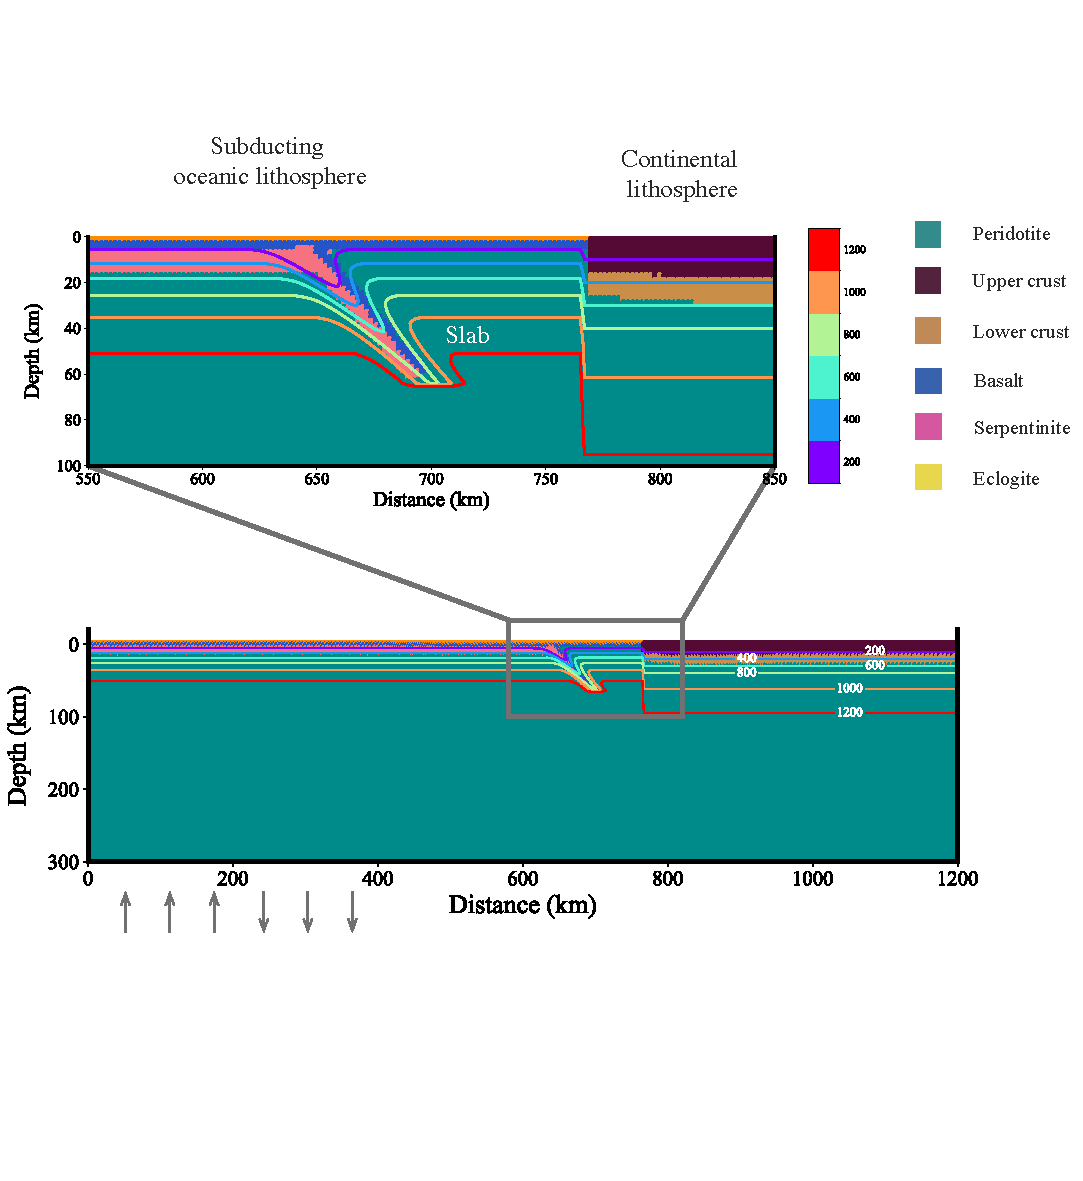
\includegraphics[width=6in]{Ref_Cocos.pdf}
    \caption[墨西哥參考模型設計與邊界條件示意圖]{墨西哥參考模型設計與邊界條件示意圖}
    \label{fig::reference Cocos model}
\end{figure*}

海洋岩石圈年齡為15個百萬年(\citealp{Manea2011Thermal}; \citealp{muller2019}),極為年輕,包含2公里厚的沉積物與6公里厚的玄武岩。由於從地球物理觀測資料得知科克斯板塊隱沒帶富含有大量水份,因此初始模型預設有10公里厚的綠泥岩,並且在隱沒過程中會產生30公里厚的蛇紋岩化橄欖岩。
海洋岩石圈熱構造由第二章式\ref{eq:Half Space Model}提及的半空間冷卻模型決定。
大陸岩石圈包含20公里厚的上部地殼(upper crust)與10公里厚的下部地殼(lower crust),過去有不少研究討論墨西哥區域的熱構造,包含穩態模擬、地磁逆推獲得居禮溫度面與熱流資料研究。本研究主要參考\citealp{Manea2011Curie}所模擬出的岩石圈熱構造,他們結合地磁逆推與隱沒帶模型模擬,推斷在40公里以上地殼地溫梯度每公里攝氏20$^{\circ}$,40公里以下地溫梯度每公里6度,至岩石圈底部為攝氏1330$^{\circ}$。模型頂部邊界溫度為攝氏10$^{\circ}$,底部邊界溫度為攝氏1330$^{\circ}$。
模型左邊界以每年7公分速率往右移動,右邊界則固定不動。
本研究參考的速度同樣來自於\citealp{o2005uncertainties},與智利參考模型相同,模型上邊界為自由表面,而下邊界則為開放邊界,物質可自由進出。

本參考模型的岩石物理特性與智利參考模型類似,除了地函橄欖岩之外有較低的活化能之外,其餘物理性直接相同。
地函橄欖岩活化能的減少造成岩石強度比原先降低10$\%$左右。


\subsection{模型結果}\label{墨西哥參考模型結果}
墨西哥參考模型產生一深度約35-40公里、長度約80-100公里的平坦段。

在隱沒初始時期,由於海洋岩石圈極為年輕,此時海洋岩石圈等深度下溫度遠高於大陸岩石圈,因此模型早期玄武岩相變位置不斷往地函深處移動,於模型5 Myr時來到接近100公里深,如圖\ref{fig::Ref Cocos 26}a。
儘管如此,大陸岩石圈厚度約為100公里,相比於普通大陸岩石圈厚度較薄、溫度較高。
地函楔中橄欖岩融點因大量自由水加入而降低,在距離海溝100公里處發生部分熔融,如圖\ref{fig::Ref Cocos 26}c中黃色線段處。
同時劇烈的脫水作用導致大量蛇紋岩化的橄欖岩在地函楔形成大範圍的低黏滯度區,如圖\ref{fig::Ref Cocos 26}b,促使地函流流動,增加地函楔溫度。
在近地表,海洋地殼上的沉積物、因變形而破碎的海洋地殼與蛇紋岩化橄欖岩在弧前區域堆積。
此時隱沒板塊以一相對高角度的狀態隱沒,角度可達50度,與正常的隱沒帶無異,隱沒角度隨時間變化如圖\ref{fig::Cocos Ref time}c。

在模型進行約略8 Myr時,隱沒板塊在深度30公里左右觸碰大陸岩石圈,隨後隱沒板塊角度開始快速下降,與動水壓力力矩顯著上升的時間點不謀而合,如圖\ref{fig::Cocos Ref time}d。
從圖\ref{fig::Ref Cocos 51}d模型動態壓力可見於地函楔頂部出現一低壓區,其與隱沒板塊下方因板塊彎曲所形成的高壓帶造成明顯的壓力梯度,因此造成動水壓力力矩增加。
同時間圖\ref{fig::Ref Cocos 51}c顯示在地函楔較深處持續發生部分熔融,在地表絕對座標700公里處有火山島弧生成。

隨後從10-15 Myr隱沒傾角逐漸降低,至接近15 Myr時模型達到平坦隱沒條件。
此時,地表上增積岩體累積厚大的沉積物,其所形成的弧前隆起高過火山島弧。
在隱沒板塊上方
這段時間隱沒板塊狀態直接影響岩漿作用特徵。
部分熔融比例幾乎呈指數減少,熔融量在平坦隱沒發育後趨近於0,暗示著火山活動停止,可見圖\ref{fig::Cocos Ref melting time}。
此外,部分熔融發生位置在5百萬年間往內陸移動超過50公里,暗示著地函楔攝氏60$^{\circ}$等溫線逐漸往內陸移動。

隨著隱沒持續進行,穩定的平坦隱沒於20 Myr後不再有明顯幾何上的改變,平坦深度維持在莫合面之下,符合墨西哥區域的接收函數結果(\citealp{PerezCampos2008}),見圖\ref{fig::Ref Cocos 101}a、圖\ref{fig::Ref Cocos 126}a與圖\ref{fig::Ref Cocos 150}a。
隱沒地殼與大陸地殼交界處有一厚度約5公里的沉積物厚層,中間夾雜些許蛇紋岩化橄欖岩,這暗示著隱沒板塊平坦段雖然有長達100公里與大陸地殼接觸,然而交界處物質強度極弱,黏滯度低,很可能無法累積大量應力。
\citealp{Song2009}、\citealp{Song2012SC}利用地震學研究,皆有觀測得平坦段上的交界層為低速層。
\citealp{Song2012SC}更藉由非均相性認為其為經歷強烈剪切的變質岩成分。
\citealp{Manea2017}則認為該弱耦合物質為殘餘的蛇紋岩。
在本參考模型中,獲得的低強度層應為沉積物主導、具有少部分蛇紋岩的岩石成分。

值得一提的是,模型時間30 Myr的壓力剖面\ref{fig::Ref Cocos 150}顯示在大陸岩石圈進地表雖然有火山島弧,然而並沒有顯著的高壓區域,為另一弱偶和特徵的展現。
反觀於智利參考模型中壓力剖面自平坦隱沒發育後(\ref{fig::Nazca_Ref_76}d至\ref{fig::Nazca_Ref_126}d)便在上覆地殼近地表出現長達150公里的高壓區,顯示平坦隱沒於智利參考模型扮演著強耦合的角色。



\begin{figure*}[htp]
    \centering
    \includegraphics[width=6in]{Cocos_a0646frame_26_snapshot_5field_150_v1.pdf}
    \caption[墨西哥參考模型於5 Myr時之結果]{墨西哥參考模型於5 Myr時之結果。}
    \label{fig::Ref Cocos 26}
\end{figure*}

\begin{figure*}[htp]
    \centering
    \includegraphics[width=6in]{Cocos_a0646frame_51_snapshot_5field_150_v1.pdf}
    \caption[墨西哥參考模型於10 Myr時之結果]{墨西哥參考模型於10 Myr時之結果。}
    \label{fig::Ref Cocos 51}
\end{figure*}

\begin{figure*}[htp]
    \centering
    \includegraphics[width=6in]{Cocos_a0646frame_76_snapshot_5field_150_v1.pdf}
    \caption[墨西哥參考模型於15 Myr時之結果]{墨西哥參考模型於15 Myr時之結果。}
    \label{fig::Ref Cocos 76}
\end{figure*}

\begin{figure*}[htp]
    \centering
    \includegraphics[width=6in]{Cocos_a0646frame_101_snapshot_5field_150_v1.pdf}
    \caption[墨西哥參考模型於20 Myr時之結果]{墨西哥參考模型於20 Myr時之結果。}
    \label{fig::Ref Cocos 101}
\end{figure*}

\begin{figure*}[htp]
    \centering
    \includegraphics[width=6in]{Cocos_a0646frame_126_snapshot_5field_150_v1.pdf}
    \caption[墨西哥參考模型於25 Myr時之結果]{墨西哥參考模型於25 Myr時之結果。}
    \label{fig::Ref Cocos 126}
\end{figure*}

\begin{figure*}[htp]
    \centering
    \includegraphics[width=6in]{Cocos_a0646frame_150_snapshot_5field_150_v1.pdf}
    \caption[墨西哥參考模型於30 Myr時之結果]{墨西哥參考模型於30 Myr時之結果。}
    \label{fig::Ref Cocos 150}
\end{figure*}

\newpage
\subsection{墨西哥參考模型脫水位置與岩漿作用}
模型中發生部分熔融與海溝之距離隨時間變化如圖\ref{fig::Cocos Ref melting time}a所示。部分熔融量隨時間變化如圖\ref{fig::Cocos Ref melting time}b。模型中共可分成三段岩漿活躍時期與一段岩漿靜止期。

第一段岩漿活躍期在0-8 Myr隱沒早期,此時熔融量不多,以地函楔中的橄欖岩為主,主要發生在距海溝100公里處,為標準的島弧岩漿特徵。
第二段岩漿活躍期出現在8-20 Myr,由於平坦隱沒在8 Myr開始發育,因此當隱沒板塊發生幾何形狀改變後,部分熔融位置開始往內陸移動,從8-15 Myr之間共移動百餘公里。
岩漿靜止期始於平坦隱沒順利成形的15 Myr,此時因隱沒板塊逐漸貼近大陸地殼下方,莫合面下的地函楔範圍逐漸縮小,因此發生部分熔融的位置不變,但比例逐漸下降,熔融量趨近於0,最終地函楔橄欖岩部分熔融比例於模型進行20 Myr時達到最小值。
\begin{figure*}[h]
    \centering
    \includegraphics[width=5in]{Ref_Cocos_melting_time_v1.pdf}
    \caption[墨西哥參考模型岩漿作用隨時間變化]{墨西哥參考模型岩漿作用隨時間變化,灰色底標出平坦隱沒發育後時間段。(a)部分熔融與海溝之距離隨時間變化圖,縱軸中每個點代表每次部分熔融發生位置,顏色為指數上的部分熔融比例。(b)岩石熔融量隨時間變化圖,熔融量單位為每單位海溝產生之立方公里量中每20萬年瞬時量。顏色代表不同岩相。}
    \label{fig::Cocos Ref melting time}
\end{figure*}

隨後模型進入第三段岩漿活躍期,在20 Myr前,部分熔融狀態有一不連續間隔,熔融位置改變、比例稍微上升,如圖\ref{fig::Cocos Ref melting time}a。
這暗示著岩漿作用區域改變,並且在該不連續時間段段後,部分熔融又重新以緩慢的速率往內陸遷移,與平坦隱沒平坦段的持續發育增長有關,隱沒板塊平坦段長度隨時間變化見圖\ref{fig::Cocos Ref time}a。
平坦隱沒具有與正常隱沒帶不同的溫壓路徑,由於其地殼在等深度下維持不變長達近80公里,在整段平坦段中壓力不變,但越靠內陸側之岩石溫度越高,此時鐵鎂岩相與沉積岩相很有可能會通過固熔點,導致海洋地殼發生部分熔融。
圖\ref{fig::Cocos Ref melting time}所統計之熔融岩相量顯示在20 Myr後陸續發生沉積物部分熔融,甚至在23 Myr後橄欖岩熔融消失,此特徵與該地區的岩漿觀測研究相符。

本參考模型的岩漿庫規模遠大於智利參考模型,累積的岩漿庫體積約是智利參考模型的100倍以上,根本原因為本研究所使用的岩漿庫冷卻參數與溫度高度相關。
在墨西哥模型中,無論海洋岩石圈或大肚岩石圈溫度梯度皆比智利參考模型高,因此岩漿庫不易冷卻,火山活動活躍。

將模型中部分熔融事件與岩漿庫絕對位置繪出,分別獲得圖\ref{fig::Cocos Ref 2Dtime series}a, b。
圖中顯示顯著的三段岩漿活躍期,第一段岩漿活躍期發生在絕對座標500至650公里、距海溝100公里之間,與正常的島弧岩漿活動特徵類似。
第二段岩漿活躍期發生在絕對座標650-750公里內,熔融深度、岩漿庫深度較第一段活躍期深,岩漿量也較大。
最終第三段岩漿活躍期發生在絕對座標750-830公里內,岩漿庫規模皆沒有前兩段活躍期大,但位置較集中,並且持續時間最長。

玄武岩至榴輝岩相變位置見圖\ref{fig::Cocos Ref 2Dtime series}c。
在模型早期,因隱沒岩石圈溫度比大陸岩石圈高,因此玄武岩至榴輝岩相變深度從40公里逐漸往接近100公里移動。
然而從圖\ref{fig::Ref Cocos 26}a與c可見儘管發生相變發生位置逐漸變深,該時期是一高角度隱沒帶,並沒有明顯的隱沒傾角趨緩特徵。
隨後在15 Myr之後,玄武岩相地殼來到模型時間段間最小長度,亦即玄武岩進入海溝後於15 Myr時會以最短的速度相變成榴輝岩相,圖\ref{fig::Cocos Ref time}d中顯示在15 Myr後重力力矩達到最高點,同樣可驗證該時間點為榴輝岩相長度達到模型中最大值,然而此時間剛好發生在平坦隱沒形成後不到一個百萬年。
因此,再次證明玄武岩相變與榴輝岩的出現仍然可以形成長久穩定的平坦隱沒。
隨後由於平坦隱沒地殼往內陸延伸的速度大於隱沒地殼增溫的速度,因此玄武岩相變深度再次往內陸推進。
平坦段中增溫速度緩慢顯示其上方沒有顯著的不可逆變形,因此摩擦熱不大,這進一步意味著平坦段上的應力狀態以低耦合為主,再次與觀測資料吻合(\citealp{moran2007cenozoic}, \citealp{PerezCampos2008})。

\begin{figure*}[ht]
    \centering
    \includegraphics[width=4in]{Cocos_a0646_2Dtime_series_v1.pdf}
    \caption[墨西哥參考模型部分熔融、岩漿庫與玄武岩相變時空關係圖]{墨西哥參考模型部分熔融、岩漿庫與玄武岩相變時空關係圖。}
    \label{fig::Cocos Ref 2Dtime series}
\end{figure*}

\newpage
\subsection{參考模型隱沒板塊與其轉動平衡}
模型中的平坦隱沒長度與深度隨時間變化見圖\ref{ffig::Cocos Ref time}a, b,平坦段深度與長度的定義已於\ref{平坦隱沒定義}節提及。

在平坦隱沒發育初期,模型時間15-20 Myr之間平坦隱沒還在緩慢發育,並且玄武岩相變深度持續加深,因此儘管重力力矩逐漸下降,平坦段長度並沒有顯著增加,隨後於20 Myr後,重力力矩不再變化,平坦段開始增長,至30 Myr可到達超過100公里長。
儘管平坦隱沒段長度逐漸變長,然而模型中平坦隱沒段深度於全時段皆沒有劇烈改變,均落在30-40公里深上下。
平坦隱沒段長度與深度皆與觀測資料吻合。

模型中隱沒板塊於150公里之內的角度變化如圖\ref{fig::Cocos Ref time}c所示。
在模型早期,角度隨時間增加直到5 Myr,隨後隨著動水壓力力矩快速增加(圖\ref{fig::Cocos Ref time}d),隱沒傾角開使緩慢下降。
在模型時間15 Myr後,隱沒傾角不再劇烈改變,暗示平坦隱沒開始發育後,隱沒帶趨近穩定,不再有幾何形狀上的變化。

\begin{figure*}[hb]
    \centering
    \includegraphics[width=4in]{Ref_Cocos_time_v1.pdf}
    \caption[墨西哥參考模型隱沒板塊狀態隨時間變化]{墨西哥參考模型隱沒板塊狀態隨時間變化。}
    \label{fig::Cocos Ref time}
\end{figure*}

模型中不同時間段的重力力矩與動水壓力力矩值如圖\ref{fig::Cocos Ref time}d。
由於本參考模型有玄武岩相變位置改變的現象,因此重力力矩在時間軸上改變劇烈。
模型早期有顯著的玄武岩相變深度變化,然而在隱沒板塊觸碰到大陸地殼後,被動導致隱沒傾角逐漸減少,玄武岩相變深度逐漸回歸至50公里深,隱沒板塊溫度逐漸升高。
重力力矩在模型時間15 Myr達到最大值,隨後隨著平坦隱沒發育,玄武岩相變位置有水平方向上的變化,逐漸往內陸移動,導致重力力矩逐漸減小。

動水壓力力矩增加起始時間早於重力力矩,應發生於隱沒板塊觸碰到大陸地殼的瞬間開始大幅增加。
在平坦隱沒發育後,動水壓力力矩雖有上升趨勢,然而增加斜率緩慢。
導致本模型能維持平坦隱沒持續15 Myr的原因可能有兩種,
第一,因為玄武岩相變深度加深的現象導致重力力矩在15 Myr後持續減少,因此平坦隱沒能穩定存在。
第二,早在動水壓力力矩巨幅增加的時期,便已經決定整個隱沒系統的動態穩定。由於15 Myr後動水壓力力矩依然有極大的轉動力矩,因此無論重力力矩是否下降,平坦隱沒皆可穩定存在。
% !TeX root = ../main.tex

\chapter{討論}

針對兩種平坦隱沒模型,各有不同的觀測資料特徵。
本章將模型結果與觀測資料進行比對,討論兩種平坦隱沒類型所具有的構造特色與岩漿作用狀態。
最後,將討論模型中可能影響平坦隱沒的形成原因。

\section{隱沒系統的耦合狀態}
隱沒板塊的耦合概念在1970年代晚期開始盛行(\citealp{uyeda1979back}; \citealp{ruff1980seismicity}),\citealp{uyeda1979back}以隱沒板塊的年紀將隱沒帶分成兩種類型:第一種是年老隱沒板塊的馬尼亞納型(Mariana type)隱沒帶,第二種是年輕隱沒板塊的智利型(Chilean type)隱沒帶,示意圖如圖\ref{fig::end-member subduction}所示。
\begin{figure*}[htp]
    \centering
    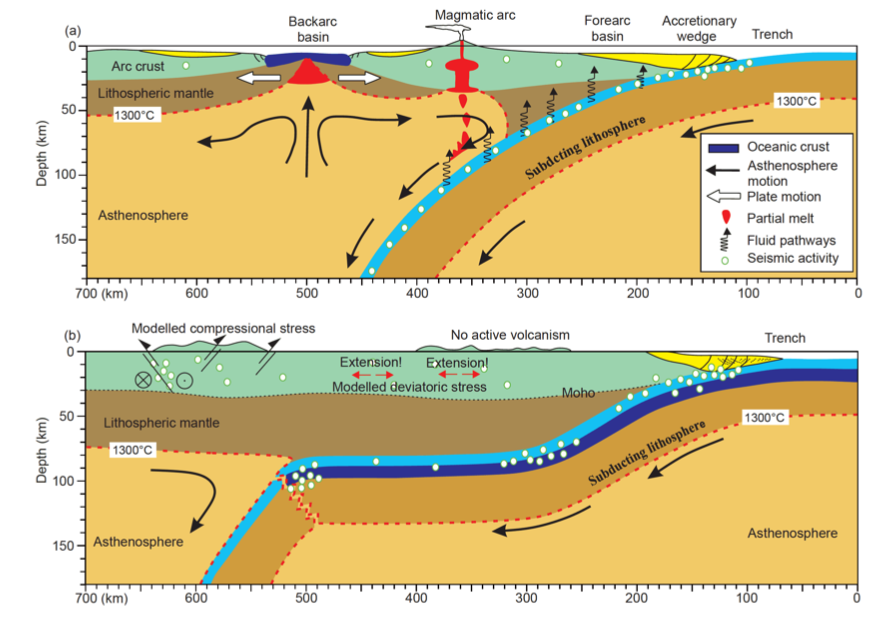
\includegraphics[width=6in]{2020subduction_type.png}
    \caption[隱沒帶的兩種型態示意圖,摘自\citealp{Yan2020}]{隱沒帶的兩種型態示意圖,摘自\citealp{Yan2020}。(a)馬尼亞納型隱沒帶(b)智利型隱沒帶}
    \label{fig::end-member subduction}
\end{figure*}

馬尼亞納型隱沒帶中隱沒板塊年紀較大、密度較大,重力較大造成隱沒板塊垂直分量上的拉力較大、隱沒傾角較高,與上覆板塊的接觸面積相對較小,可見圖\ref{fig::end-member subduction}a。
此類隱沒帶的應力不易累積,容易發生潛移活動,地震事件規模較小且通常為伸張地震,故馬尼亞納型隱沒帶又可稱為弱耦合(weak coupling)隱沒帶。
此外,高角度的隱沒板塊造成地函楔容易發生強烈對流,伴隨隱沒帶的部分熔融作用,在上覆板塊側發生拉張現象,可能會產生弧後張裂(back-arc spreading)(\citealp{lallemand2005relationships})。
反之智利型隱沒帶因隱沒板塊溫度較高、密度較小,故隱沒傾角較低,在聚合板塊交界處產生較大的板塊接觸面積,如圖\ref{fig::end-member subduction}b。
通常此類隱沒帶會容易產生低角度的班尼奧夫帶,地震事件多以逆衝斷層為主,且發生過多起大規模(Mw>8.0)地震事件(\citealp{uyeda1979back})。
上覆板塊側有顯著的壓縮應力(\citealp{hu2021southward}),可能會在弧後出現許多皺褶與斷層,因此智利型隱沒帶亦會被視為強耦合(strong coupling)隱沒帶。

\subsection{智利平坦隱沒的耦合狀態}
過去的研究注意到智利上覆板塊的地殼地震事件數目在平坦隱沒區域較多(\citealp{jordan1983andean}; \citealp{smalley1993basement}),表明平坦隱沒區域具有比正常隱沒帶更強的板塊間耦合。
\citealp{gutscher2002andean}統計智利沿岸在距海溝250-800公里的所有地震事件所釋放之能量總和,以南北向一度以內為單位,獲得板塊釋放的地震能量直方圖(見圖\ref{fig::Chile_seismicity})。
總體而言,智利中部平坦隱沒上方的板塊所釋放出的地震能量比北部玻利維亞段高出5倍,比南段智利高出10倍。
\citealp{jordan1983andean}分析智利沿岸大地震的震源機制解,顯示該區域以壓縮型地震主導,他認為隱沒邊界應力有效傳遞到上覆板塊,並且在平坦隱沒段有更高程度的板塊間耦合。

\begin{figure*}[htp]
    \centering
    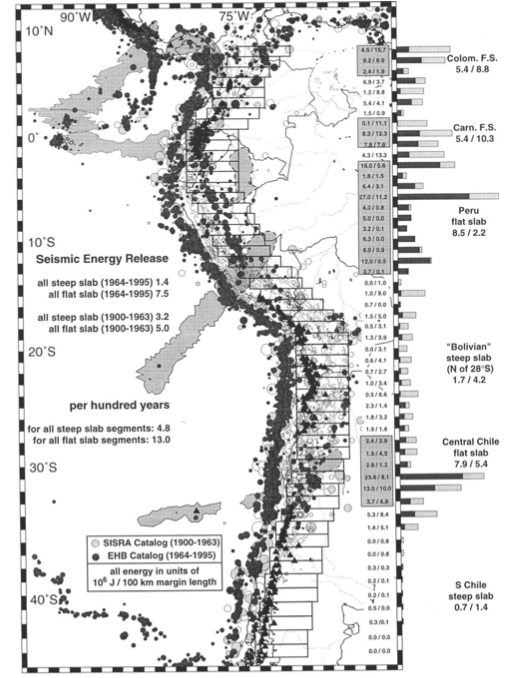
\includegraphics[width=5in]{Seismicity and Energy of Andes.png}
    \caption[智利沿岸自21$^\circ$S到44$^\circ$S的上板塊地震活動統計分析,摘自\citealp{gutscher2002andean}]{智利沿岸自20$^\circ$S到40$^\circ$S的上板塊地震活動統計分析,摘自\citealp{gutscher2002andean}。這裡採用深度<70公里的地震事件總能量,單位為10$^6$焦耳。右側數字表示1900-1963年/1964-1995年間所示分的地震能量。數字下灰色底框標示出平坦隱沒段的位置。
    }
    \label{fig::Chile_seismicity}
\end{figure*}

本研究智利參考模型的水平應力(Sxx)剖面圖如圖\ref{fig::Sxx_and_Pressure_Chile}a所示。
其中,水平應力大於0表示拉張,水平應力小於0表示壓縮。
上覆板塊側的水平應力在平坦隱沒段上地殼處有較小值,表示壓縮應力的存在。
上覆板塊的壓縮應力在水平方向上可分為兩區域,第一個區域位在近地表30公里以上、絕對座標550-650公里之間,其下方對應到隱沒板塊上凹變形處位置。
第二個區域較不明顯,位於絕對座標750-800公里、深度50-70公里處,對應到隱沒板塊下傾位置。
動水壓力剖面同樣可以觀察到類似的現象,在圖\ref{fig::Sxx_and_Pressure_Chile}b中,上覆板塊淺層於絕對座標550-650公里處有很大的正壓力,與圖\ref{fig::Sxx_and_Pressure_Chile}a中的壓縮應力位置相似。

\begin{figure*}[h]
    \centering
    \includegraphics[width=5.5in]{Sxx_and_Pressure_Chile_of_201.pdf}
    \caption[智利參考模型於40 Myr的水平軸差應力與動水壓力剖面]{智利參考模型於40 Myr的水平軸差應力與動水壓力剖面,其中應力正向代表拉張應力,負向代表壓縮應力。}
    \label{fig::Sxx_and_Pressure_Chile}
\end{figure*}
\subsection{墨西哥平坦隱沒的耦合狀態}
儘管如此,墨西哥平坦隱沒並沒有強耦合的特徵。
\citealp{PerezCampos2008}的接收函數結果顯示墨西哥的隱沒板塊平坦段深度直接位於莫荷面下方,因此隱沒板塊與上覆板塊的接觸面材質為海洋地殼與下部大陸地殼的成分,幾乎不包含任何大陸地函軟流圈(continental mantle asthenosphere),此時板塊介面在聚合過程中理論上應產生很大的摩擦力。
此外,墨西哥隱沒帶被視為侵蝕型隱沒(subduction erosion)(\citealp{stern2011subduction}),其證據包含現今外海的沉積物厚度約200公尺(\citealp{manea2003sediment}),並且擁有快速的聚合速率(\citealp{o2005uncertainties})。
再配合年輕隱沒帶的低傾角隱沒特徵,墨西哥平坦段聚合板塊接觸面積極大。
種種物理跡象表明該區域應該為強耦合環境。
然而墨西哥平坦隱沒段的地震活動度極低,格雷羅無震帶(\citealp{kostoglodov2003large})便位於平坦段上,表明平坦段並非處於強耦合狀態。
除此之外,平坦隱沒上方並沒有顯著的水平壓縮現象(\citealp{nieto2006latest}; \citealp{moran2007cenozoic},這與強耦合的特徵互相矛盾。
對此,\citealp{Manea2011Thermal}模擬墨西哥平坦隱沒剖面的熱構造。
隱沒板塊段上海洋地殼與沉積物絕大部分在距海溝250公里前便完成脫水,大量的水分可能釋放進入下大陸地殼中,導致岩石強度降低,不容易累積大量應力。
該地區的非火山微震(non volcanic tremor)發生位置與海洋地殼的脫水位置相吻合\citealp{Manea2011Thermal},慢地震(slow slip event)事件位置則與沉積物的脫水位置吻合\citealp{Song2009}。
大量的微震與慢地震事件暗示著該區域為弱耦合隱沒帶。

本研究墨西哥參考模型的水平應力(Sxx)剖面圖如圖\ref{fig::Sxx_and_Pressure_Mexico}a所示。
上覆板塊側的水平應力在上部地殼與下部地殼底部各有一層高區。
此外,在絕對座標700公里與800公里處的火山島弧下方也具有地區性的水平應力小值,其為火山形成的荷重所造成。
與智利參考模型相比,墨西哥參考模型的上覆版塊沒有顯著的壓縮應力存在。
動水壓力剖面同樣可以觀察到類似的現象,如圖\ref{fig::Sxx_and_Pressure_Mexico}b所示,上覆板塊側除了上下地殼交界處與莫荷面處有較高的正壓力外,並沒有顯著來自隱沒板塊介面所提供的正壓力。
\begin{figure*}[ht!]
    \centering
    \includegraphics[width=5in]{Sxx_and_Pressure_Phase_Mexico_of_201_v5.pdf}
    \caption[墨西哥參考模型中於40 Myr的剖面]{墨西哥參考模型中於40 Myr的水平軸差應力、動水壓力與岩相剖面。(a)水平軸差應力剖面,其中應力正向代表拉張應力,負向代表壓縮應力。(b)動水壓力剖面。(c)模型岩相剖面,岩相顏色請見圖\ref{fig::Ref Cocos 26}。}
    \label{fig::Sxx_and_Pressure_Mexico}
\end{figure*}

本研究於第\ref{墨西哥隱沒帶地球物理觀測}節與第\ref{墨西哥參考模型結果}節皆有提及地震學研究在墨西哥平坦隱沒區域的板塊介面中發現一層低速層(\citealp{PerezCampos2008}),\citealp{Song2009}估計該低速層厚度約3-5公里且V$_S$速度約每秒2-2.7公里,大約降低26-40$\%$左右。
過去對於該低速層的成分有諸多解釋,\citealp{Song2012SC}認為其為經歷強烈剪切的變質岩成分。
\citealp{Manea2017}則認為該弱耦合物質為殘餘的蛇紋岩。

從墨西哥參考模型的岩相圖\ref{fig::Sxx_and_Pressure_Mexico}c可見隱沒板塊與大陸地殼的介面中具有厚度4-8公里、以沉積岩為主參雜少許蛇紋岩化橄欖岩的弱物質。
由於該弱物質層的岩石強度極弱,故隱沒板塊介面成為弱耦合介面,上覆板塊的壓縮應力較小。
因此,並非所有低傾角隱沒帶皆具有強耦合的特徵。

\section{平坦隱沒中的埃達克岩}\label{平坦隱沒中的埃達克岩}
埃達克岩(adakite)最初由\citealp{kay1978aleutian}觀測阿留申群島中Adak Island上一種高La/Yb、高Sr/Y以及富含大離子半徑元素(large ion lithophile (LIL)- element-rich)的安山岩,其特徵與一般的火山島弧安山岩不相同,爾後\citealp{defant1990derivation}將其命名為埃達克岩。
由於埃達克岩具有特殊的全岩地球化學性質,一般多半利用Sr/Y-Y作圖與(La/Yb)$_N$-Yb$_N$作圖區別埃達克岩與一般的島弧中酸性安山岩,如圖\ref{fig::AdakiteY}。

\begin{figure*}[h]
    \centering
    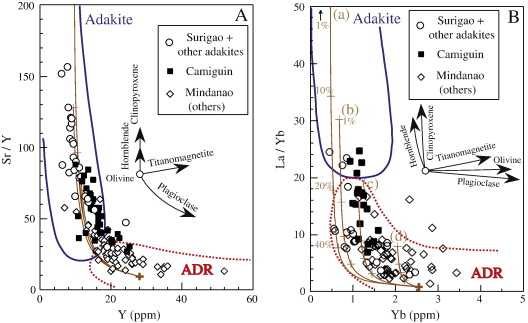
\includegraphics[width=5in]{AdakiteY.jpg}
    \caption[Sr/Y-Y作圖與(La/Yb)$_N$-Yb$_N$作圖]{(A)Sr/Y-Y作圖與(B)(La/Yb)$_N$-Yb$_N$作圖,摘自\citealp{castillo2012adakite}。通常用於區分埃達克岩與普通島弧安山岩、石英岩與流紋岩(normal arc andesite, dacite and rhyolite, ADR)。紫色實線邊界來自於\citealp{richards2007special}所提出菲律賓中南部埃達克岩與普通島弧安山岩的資料。}
    \label{fig::AdakiteY}
\end{figure*}

早期認為埃達克岩是年輕的(< 7 Ma)隱沒海洋玄武岩發生部分熔融產生的中酸性火山岩(\citealp{defant1990derivation}; \citealp{peacock1994partial})。
由於埃達克岩的定義來自岩石化學組成分定量分析,隨著相關研究累積,顯示高壓變質基性岩的部分熔融皆具有埃達克岩的特徵,
因此埃達克岩性質的火成岩可已在多種不同地體環境下產生(\citealp{martin2005overview}),以下列出最常見的四種:

(1)隱沒海洋地殼的熔融(\citealp{defant1990derivation}),隨後埃達克岩中的低Nd、高Sr同位素特徵被認為是隱沒海洋沉積物參與部分熔融所產生(\citealp{stern1996role}; \citealp{gomez2003temporal}),又有人稱其為high-SiO$_2$ adakites (\citealp{martin2005overview})。

(2)增厚大陸下地殼底部的基性岩熔融(\citealp{kay1996magmatic})。
在高壓環境下,基性岩密度過高時無法穩定存在於大陸地殼底部,因此部分熔融產生。
通常需要長時間的地殼增厚(\citealp{kay2002magmatism})才會形成高壓下的高密度基性岩,因此這種形成機制比較可能會發生在島弧岩漿作用事件中末期。

(3)普通島弧安山岩受地殼成分污染,導致岩漿混合,其稱為low-SiO$_2$ adakites (\citealp{martin2005overview}),與(1)成因中的high-SiO$_2$ adakites相對。
此埃達克岩具有較高的地函組成相關元素(MgO、K、Nb、Cr、Ni等)。

(4)來自一般的島弧基性岩漿於高壓(> 12 kbar)環境下,以石榴子石為主的結晶分化產物(\citealp{moyen2009high}),例如菲律賓蘇里高半島的埃達克岩。

一般來說,上述成因中,只有(1)與(2)兩種成因可被稱為埃達克岩,而(3)與(4)所產生之高Sr/Y類似因物質交換而繼承埃達克岩特徵,稱作類埃達克岩(Adakite-like rocks)(\citealp{kay2002magmatism}; \citealp{goss2013andean})。

早期在南美洲的平坦隱沒區域發現部分埃達克岩的紀錄,\citealp{Gutscher2000Bcan}為此提出一概念模型,為平坦隱沒特殊的溫壓條件所生成埃達克岩。
如同\ref{墨西哥參考模型脫水位置與岩漿作用}節所提及,平坦隱沒具有與正常隱沒帶不同的溫壓路徑,如圖\ref{fig::Flat slab PT}中所繪,此時鐵鎂岩相與沉積岩相很有可能會通過固熔點,導致海洋地殼發生部分熔融。

\begin{figure*}[ht!]
    \centering
    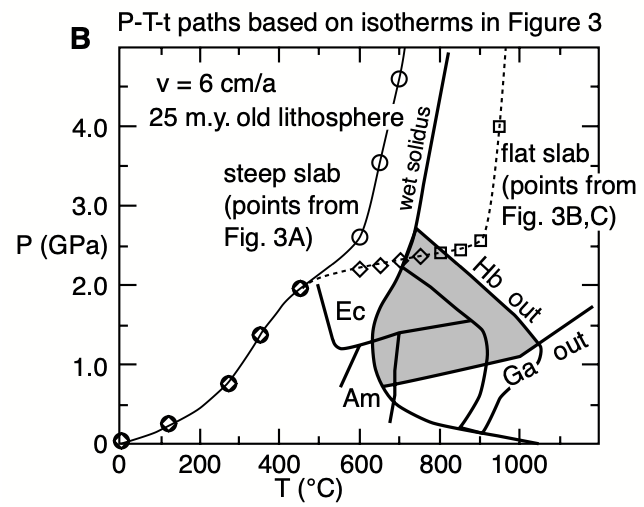
\includegraphics[width=4in]{Flat slab PT.png}
    \caption[隱沒板塊頂部可能的溫壓路徑圖,摘自\citealp{Gutscher2000Bcan}]{隱沒板塊頂部可能的溫壓路徑圖,摘自\citealp{Gutscher2000Bcan}。Ec—榴輝岩(eclogite),Am—角閃岩(amphibolite),Ga—石榴石(garnet),Hb—角閃石(hornblende)。
    圓形為正常隱沒帶中的溫壓路徑,菱形與正方形則為平坦隱沒的溫壓路徑。其中,灰色底部分為隱沒板塊可能的部分熔融區。
    }
    \label{fig::Flat slab PT}
\end{figure*}

\subsection{墨西哥平坦隱沒的岩漿作用}
在墨西哥,地球化學上所認定的埃達克岩的特徵之一為高Gd/Yb與高SiO$_2$,如圖\ref{fig::Cocos_geochemisty}b與圖\ref{fig::Cocos_geochemisty}c所示。
跨墨西哥火山帶最初於早中新世(約19 Ma)開始噴發,主要為亞鹼性(sub-alkaline)岩石,由安山岩和英安岩組成,隨著火成岩噴發位置離海溝越來越遠,地球化學特徵表明越往北(遠離海溝)的火成岩,隱沒帶中的流體量越少(\citealp{ferrari2012dynamic})。
這個趨勢在15 Ma左右被侵入的埃達克岩中斷(\citealp{mori2007effects}),見圖\ref{fig::Cocos_geochemisty}a紅色與藍色點,值得注意的是,具有埃達克岩特徵的樣本幾乎都與海溝距離超過400公里。
目前學界一致認同墨西哥平坦隱沒區域所發現的埃達克岩樣本皆為隱沒海洋地殼與沉積物的產物(\citealp{Gutscher2000Bcan}; \citealp{ferrari2012dynamic}; \citealp{Manea2017})。

\begin{figure*}[ht!]
    \centering
    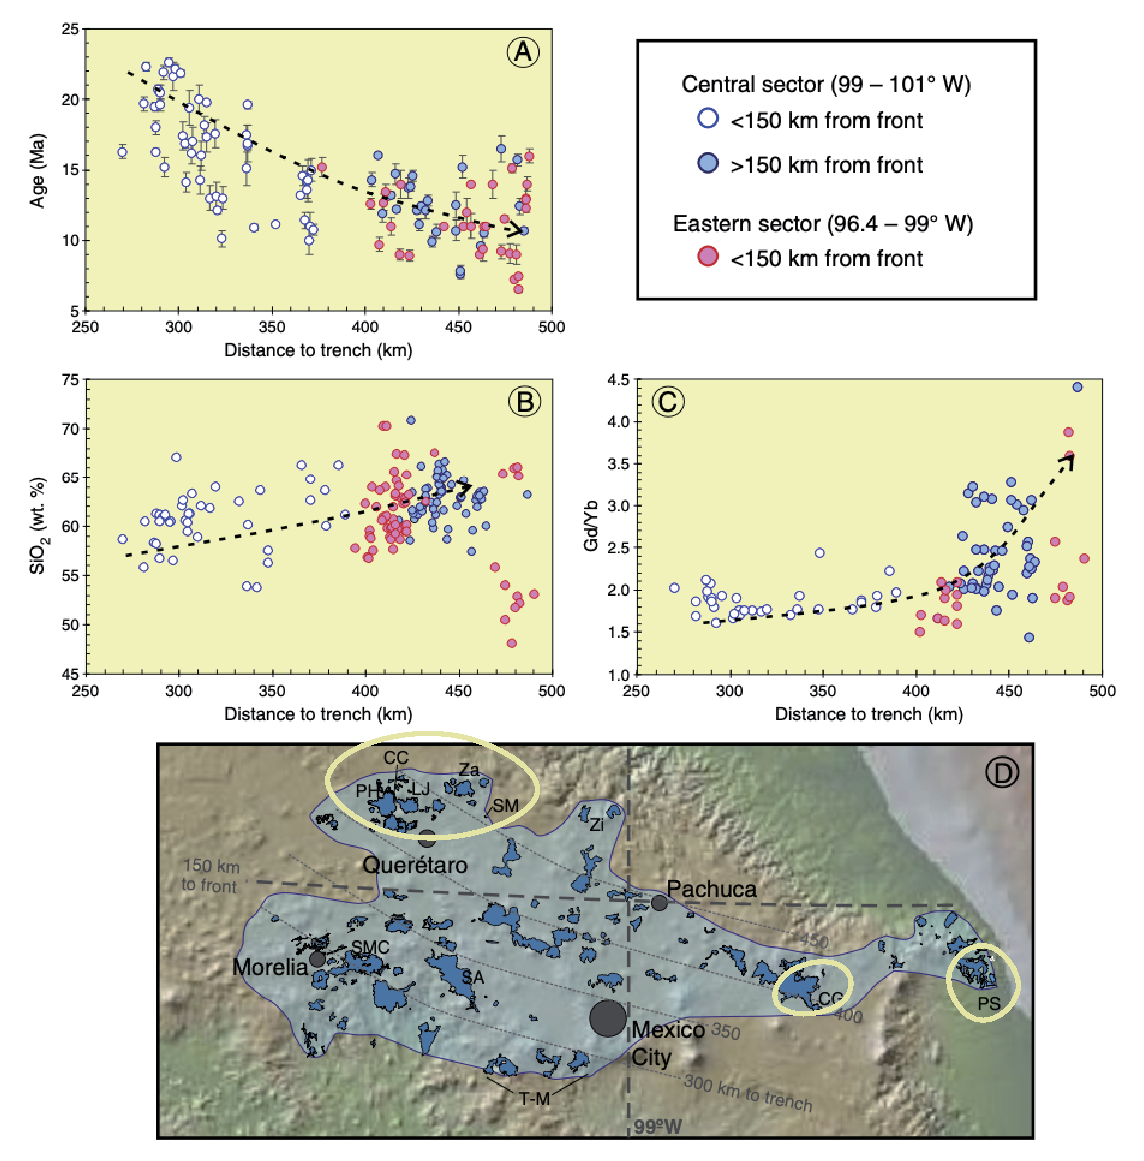
\includegraphics[width=5in]{Cocos_Volcano_v2.pdf}
    \caption[墨西哥區域火山島弧地球化學分析,摘自\citealp{ferrari2012dynamic}]{墨西哥區域火山島弧地球化學分析,摘自\citealp{ferrari2012dynamic}。白點為距現今火山弧前緣小於150公里的樣本,藍色點為具現今火山弧前緣大於150公里且位在西經99-101$^{\circ}$的樣本,紅色點為具現今火山弧前緣小於150公里且位在西經96.4-99$^{\circ}$的樣本。(a)火成岩樣本年紀與現今海溝距離作圖。(b)火成岩樣本中的SiO$_2$含量與現今海溝距離作圖。(c)火成岩樣本中Gd/Yb比值與現今海溝距離作圖。(d)墨西哥中新世火山位置圖。細虛線表示到海溝的距離,粗虛線是\ref{平坦隱沒中的埃達克岩}圖例中使用的邊界。 CC: Cerro Colorado dome,CG: Cerro Grande volcan塞羅格蘭德火山, LJ: La Joya volcan拉霍亞火山, PH: Palo Huérfano 火山, PS: Palma Sola帕爾馬索拉,SA: Sierra de Angangueo塞拉利昂德安甘格奧, SM: San Martín聖馬丁, SMC: Sierra de Mil Cumbres, T-M: Tenancingo–Malinalco特南寧哥-馬利納爾科, Za: Zamorano volcano薩莫拉諾火山, Zi: Zimapán area Zimapán 地區。
    }
    \label{fig::Cocos_geochemisty}
\end{figure*}

在墨西哥參考模型中,確實有海洋地殼部分熔融的現象。
圖\ref{fig::Cocos Ref melting time}b、c中顯示平坦隱沒形成、於模型時間15 Myr前後開始發生榴輝岩的部分熔融。
榴輝岩的部分熔融比例在平坦隱沒形成初期快速增加,在15-20 Myr之間可達50-70$\%$。
在20 Myr後,榴輝岩的部分熔融比例維持5-20$\%$之間,在時間軸上沒有太大改變。
然而沉積物自23 Myr後便成為墨西哥參考模型熔融源的主導岩石。
儘管多數研究已證實隱沒沉積物大量熔融的存在(\citealp{van2011subduction}; \citealp{Forster2021}),本研究認為該結果需要進一步確認。
本研究中,所選用的沉積物固相線為飽和水固相線(\citealp{van2011subduction}),然而模型中並沒有考量各岩石的含水量多寡,因此部分熔融的形成機制需要更多考量。

\citealp{stern1996role}針對埃達克岩樣本進行分析,表示埃達克岩中約有35-90$\%$的隱沒板塊質量,包含玄武岩、榴輝岩與沉積物。
圖\ref{fig::melting_eclogite_ratio}是墨西哥參考模型在時間軸上岩漿熔融源與熔融量變化圖,只關注於平坦隱沒發生後的岩石熔融。
圖\ref{fig::melting_eclogite_ratio}b顯示模型中榴輝岩的熔融比例與岩漿庫體積,在平坦隱沒剛形成時(15-20 Myr),所有熔融岩中,有超過40$\%$為榴輝岩,爾後榴輝岩體積比例維持10-20$\%$。
由於本研究並沒有考慮大陸地殼中的岩漿作用,以及岩漿內物質置換、結晶分異作用與岩石含水量對岩漿庫的影響,因此無法充分說明模型中所產生的火山島弧是否確切為埃達克岩的成分。
然而從模型中岩漿作用熔融源分析可證明(見圖\ref{fig::melting_eclogite_ratio}a),隱沒板塊物質確實可以發生熔融。

圖\ref{fig::Mexico_arc_location}顯示墨西哥參考模型中地表出現兩處的火山島弧。
第一處的火山島弧出現於距海溝130-180公里處,可以對應至圖\ref{fig::Cocos Ref 2Dtime series}b中的第二區岩漿庫(Magma Chamber 2)。
第二處的火山島弧出現於距海溝260-280公里處,可以對應至圖\ref{fig::Cocos Ref 2Dtime series}b中的第三區岩漿庫(Magma Chamber 3)。
本研究所產生的火山島弧與海溝距離不及圖\ref{fig::Cocos_geochemisty}中的墨西哥火山島弧,不過確實可獲得沿海溝距離上火成岩成分的劇烈變化結果。

\begin{figure*}[ht!]
    \centering
    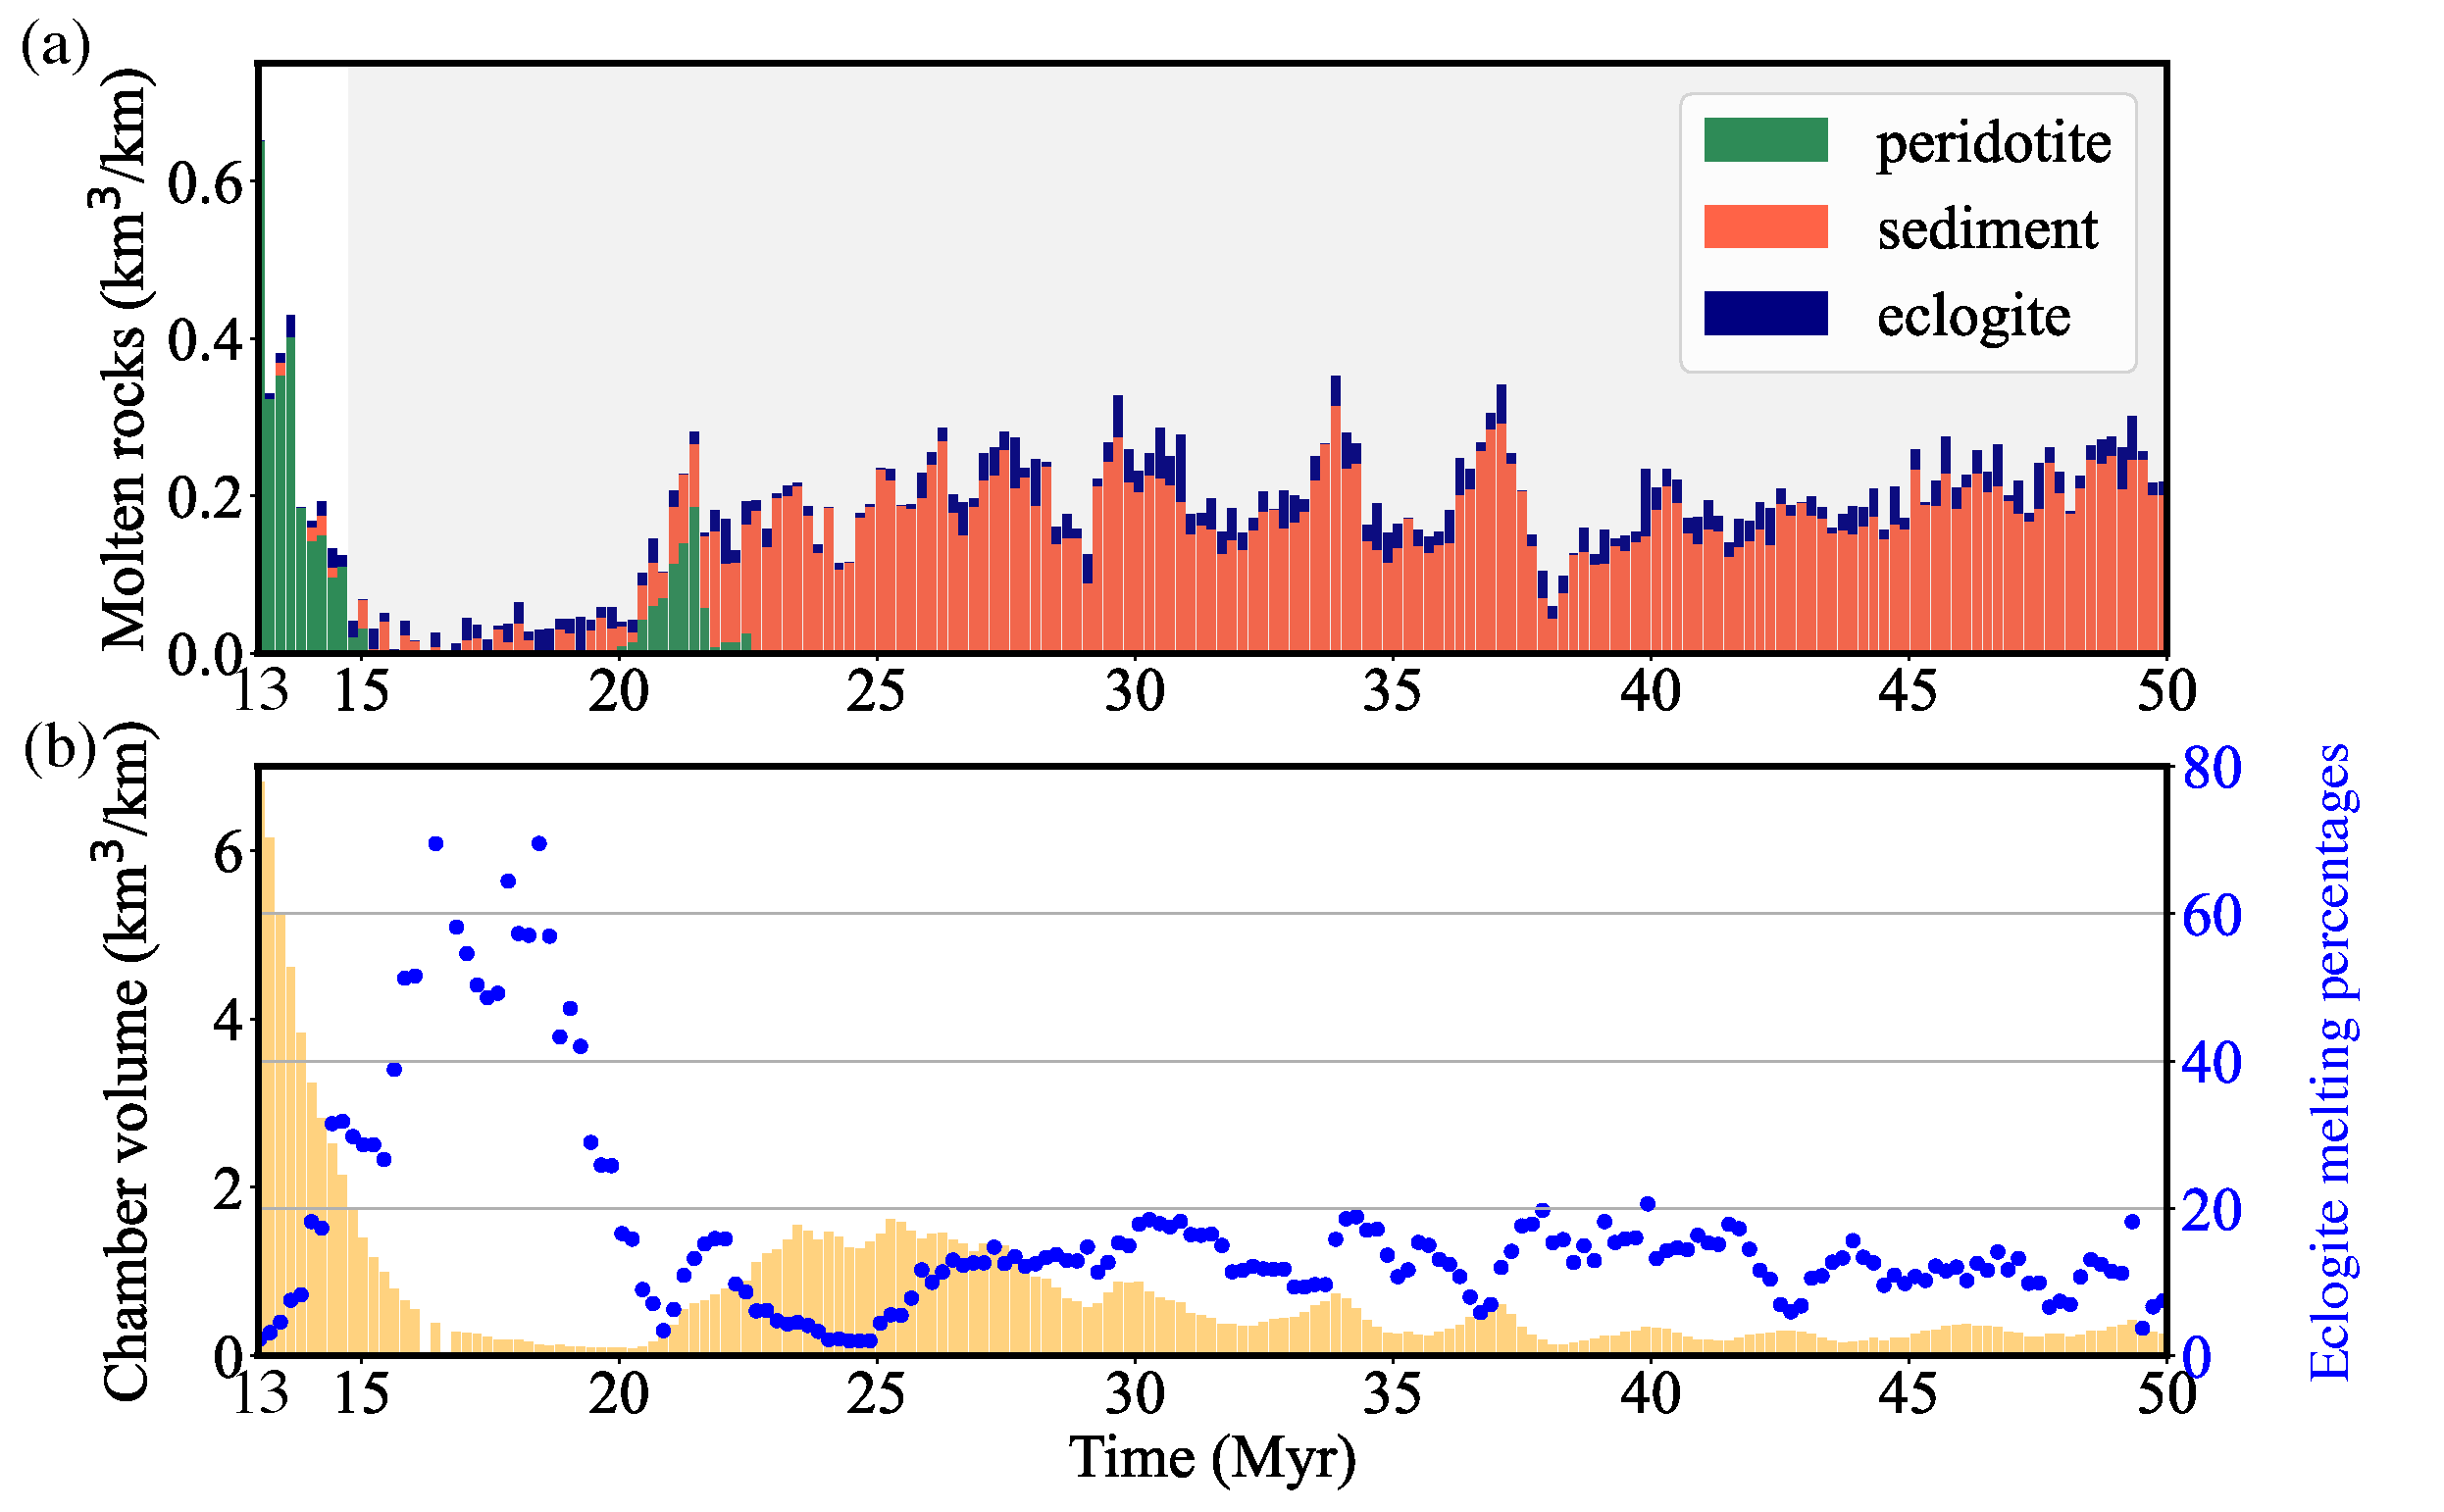
\includegraphics[width=6in]{slab_melting.pdf}
    \caption[墨西哥參考模型部分熔融源岩與岩漿庫分析]{墨西哥參考模型部分熔融源岩與岩漿庫分析。(a)同圖\ref{fig::Cocos Ref melting time}b,聚焦在13-40 Myr時期的部分熔融源岩,熔融量單位為每單位海溝產生之立方公里量中每20萬年瞬時量,模型中包含橄欖岩(綠色)、沉積岩(橘色)與榴輝岩(深藍色)熔融。灰底為平坦隱沒發生時間。(b)黃底柱狀為岩漿庫體積,藍點為榴輝岩瞬時熔融體積佔整體瞬時熔融體積的比例。
    }
    \label{fig::melting_eclogite_ratio}
\end{figure*}

\begin{figure*}[ht!]
    \centering
    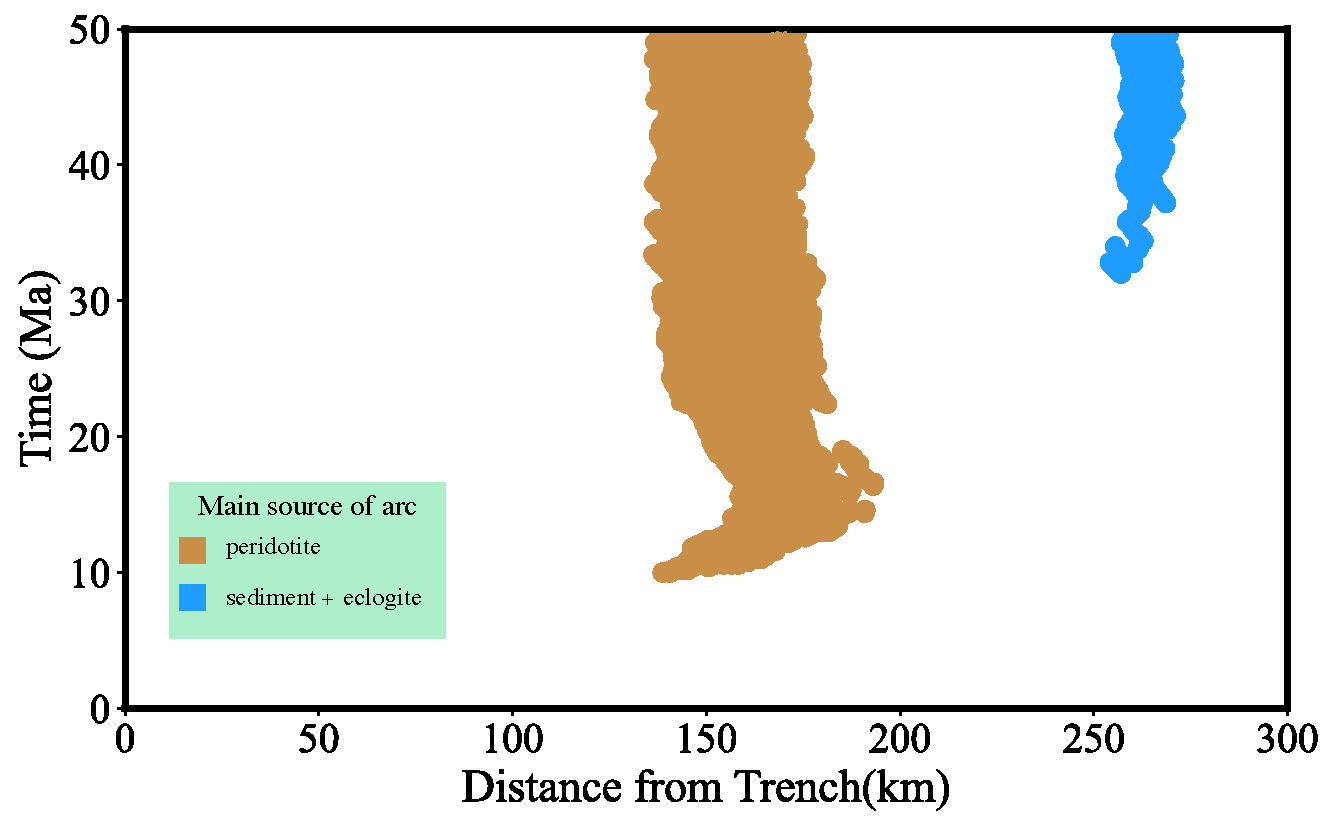
\includegraphics[width= 5in]{Mexico_arc_location_v1.pdf}
    \caption[墨西哥參考模型火山島弧與海溝距離隨時間變化]{墨西哥參考模型火山島弧與海溝距離隨時間變化。其中咖啡色為熔融源岩以橄欖岩為主的火山島弧,藍色則為熔融源岩以沉積物與榴輝岩為主的火山島弧。
    }
    \label{fig::Mexico_arc_location}
\end{figure*}

\newpage
\subsection{智利平坦隱沒的岩漿作用}

\citealp{Gutscher2000Bcan}認為南美洲平坦隱沒區域所出露的埃達克岩為隱沒板塊熔融的產物,在他們的研究中僅使用概念模型解釋埃達克岩成因,然而\citealp{kay2002magmatism}近一步對埃達克岩樣本進行地球化學分析,他們認為智利區域的埃達克岩為上述成因中的第(3)種,埃達克岩漿來自於普通島弧安山岩漿與地殼熔融發生岩漿混合,是為low-SiO$_2$ adakites。
由於本研究並沒有考慮大陸地殼成分岩石發生部分熔融,因此無法從參考模型中獲得\citealp{kay2002magmatism}所認為的結果。
然而,將智利參考模型隱沒地殼頂部溫壓狀態與隱沒板塊相圖比較(見圖\ref{fig::chile_slab_PT}),隱沒板塊並沒有通過隱沒板塊含水固相線。
此外,智利參考模型的平坦深度在100公里左右,圖\ref{fig::chile_slab_PT}中壓力維持不變且溫度持續增加的範圍落在3 GPa與攝氏500-800 $^{\circ}$之間,圖\ref{fig::Flat slab PT}中\citealp{Gutscher2000Bcan}的概念模型平坦段範圍落在2.5 GPa與攝氏400-900$^{\circ}$,兩者有顯著差異。
以智利平坦隱沒區的平坦段深度100公里來看,智利參考模型的結果較接近真實情形。
這說明本研究可以藉由排除\citealp{Gutscher2000Bcan}中所認為的埃達克岩形成方式。

\begin{figure*}[ht!]
    \centering
    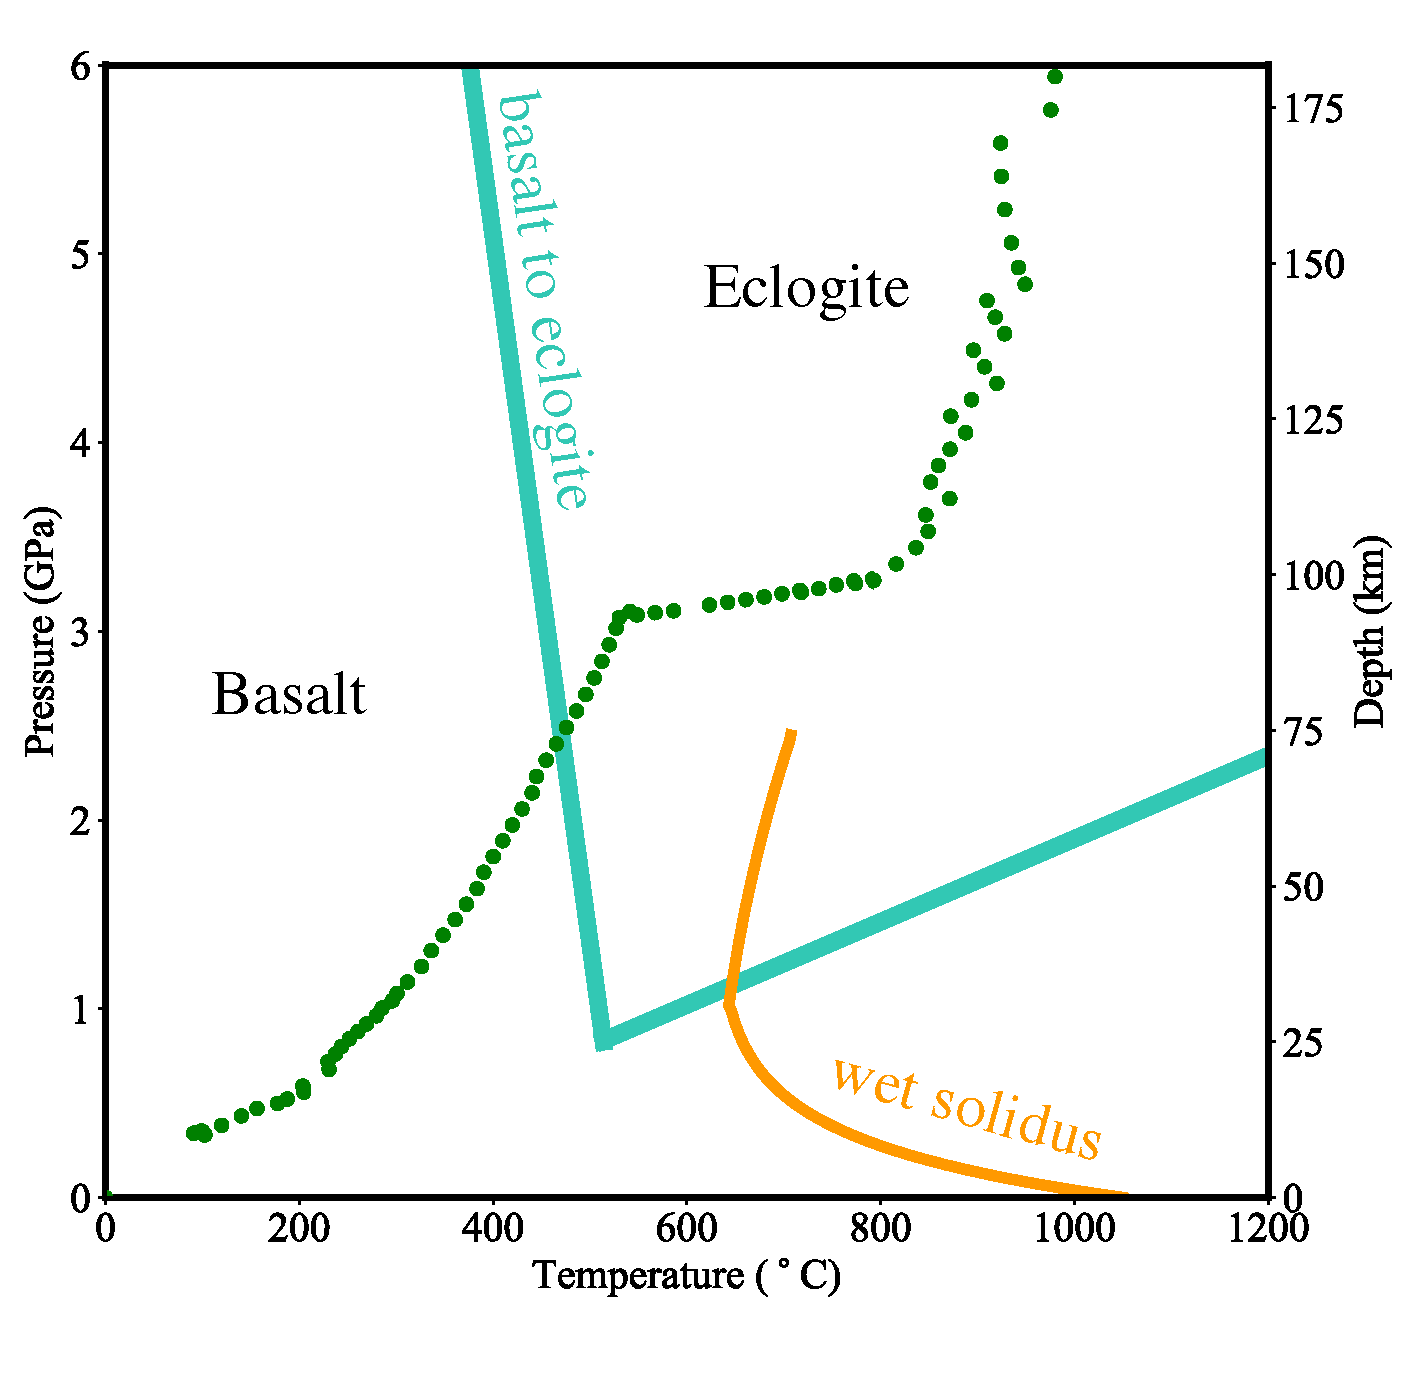
\includegraphics[width=4in]{chile_slab_PT_v1.pdf}
    \caption[智利參考模型隱沒地殼頂部於40 Myr的溫壓圖]{智利參考模型隱沒地殼頂部於40 Myr的溫壓圖。其中綠線為本研究中玄武岩至榴輝岩的相變條件,橘色線為含水固相線。綠色點為隱沒地殼頂部每2-5公里的溫壓狀態。
    }
    \label{fig::chile_slab_PT}
\end{figure*}

\newpage
\section{為什麼會形成平坦隱沒}
由於平坦隱沒的形成原因至今依然是一開放性問題,以下將討論隱沒帶中不同構造區對隱沒系統的影響,以及本研究模型中產生平坦隱沒的可能關鍵原因。
本節測試一系列數值模型參數,模型參數表見表\ref{模型參數列表}。

\begin{table}[htp]\large
    \caption[模型參數列表]{模型中參數列表}
    \label{模型參數列表}
    \renewcommand{\arraystretch}{1.2}
    \centering
    \begin{tabular}{|lllll|}
        \hline
        \multicolumn{5}{|c|}{a Upper Plate Thickness}                                                 \\ \hline
        model        & P$_0$                   & $\lambda_0$             & thickness & serpentinite \\ \hline
        Nazca\_a01 & 4.5 $\times$ 10$^{-15}$ & 1.6 $\times$ 10$^{-12}$ & 120       & 5            \\
        Ref\_Nazca   & 4.5 $\times$ 10$^{-15}$ & 1.6 $\times$ 10$^{-12}$ & 130       & 5            \\
        Nazca\_a02 & 4.5 $\times$ 10$^{-15}$ & 1.6 $\times$ 10$^{-12}$ & 140       & 5            \\
        Nazca\_a03 & 4.5 $\times$ 10$^{-15}$ & 1.6 $\times$ 10$^{-12}$ & 150       & 5            \\
        Nazca\_a04 & 4.5 $\times$ 10$^{-15}$ & 1.6 $\times$ 10$^{-12}$ & 160       & 5            \\ \hline
        \multicolumn{5}{|c|}{Serpentinite Thickness}                                                \\ \hline
        model        & P$_0$                   & $\lambda_0$             & thickness & serpentinite \\ \hline
        Nazca\_b01 & 4.5 $\times$ 10$^{-15}$ & 1.6 $\times$ 10$^{-12}$ & 130       & 2.5          \\
        Ref\_Nazca   & 4.5$\times$ 10$^{-15}$  & 1.6 $\times$ 10$^{-12}$ & 130       & 5            \\
        Nazca\_b02 & 4.5 $\times$ 10$^{-15}$ & 1.6 $\times$ 10$^{-12}$ & 130       & 7.5          \\
        Nazca\_b03 & 4.5 $\times$ 10$^{-15}$ & 1.6 $\times$ 10$^{-12}$ & 130       & 10           \\
        Nazca\_b04 & 4.5 $\times$ 10$^{-15}$ & 1.6 $\times$ 10$^{-12}$ & 130       & 15           \\ \hline
        \multicolumn{5}{|c|}{Magma Parameters}                                                      \\ \hline
        model        & P$_0$                   & $\lambda_0$             & thickness & serpentinite \\ \hline
        Ref\_Nazca   & 4.5 $\times$ 10$^{-15}$ & 1.6 $\times$ 10$^{-12}$ & 130       & 5            \\
        Nazca\_c01 & 4.5 $\times$ 10$^{-14}$ & 1.6 $\times$ 10$^{-12}$ & 130       & 5            \\
        Nazca\_c02 & 4.5 $\times$ 10$^{-13}$ & 1.6 $\times$ 10$^{-12}$ & 130       & 5            \\
        Nazca\_c03 & 4.5 $\times$ 10$^{-15}$ & 1.6 $\times$ 10$^{-13}$ & 130       & 5            \\
        Nazca\_c04 & 4.5 $\times$ 10$^{-14}$ & 1.6 $\times$ 10$^{-13}$ & 130       & 5            \\
        Nazca\_c05 & 4.5 $\times$ 10$^{-13}$ & 1.6 $\times$ 10$^{-13}$ & 130       & 5            \\
        Nazca\_c06 & 4.5 $\times$ 10$^{-15}$ & 1.6 $\times$ 10$^{-14}$ & 130       & 5            \\
        Nazca\_c07 & 4.5 $\times$ 10$^{-14}$ & 1.6 $\times$ 10$^{-14}$ & 130       & 5            \\
        Nazca\_c08 & 4.5 $\times$ 10$^{-13}$ & 1.6 $\times$ 10$^{-14}$ & 130       & 5            \\
        Nazca\_c09 & 4.5 $\times$ 10$^{-15}$ & 1.6 $\times$ 10$^{-15}$ & 130       & 5            \\
        Nazca\_c10 & 4.5 $\times$ 10$^{-14}$ & 1.6 $\times$ 10$^{-15}$ & 130       & 5            \\
        Nazca\_c11 & 4.5 $\times$ 10$^{-13}$ & 1.6 $\times$ 10$^{-15}$ & 130       & 5            \\ \hline
    \end{tabular}
\end{table}

\subsection{均質的隱沒板塊}
本研究的兩種參考模型中,隱沒板塊上皆不存在任何非均質(heterogeneous)構造或任何例外的物理特性。
同\ref{平坦隱沒的數值模型}所述,過去的數值模型提出許多降低隱沒系統重力力矩的可能原因,包含加入一段不會發生玄武岩相變的海洋地殼(\citealp{Liu2016}; \citealp{Gerya2009})、延後榴輝岩相的相變時間(\citealp{van2002role})、增厚隱沒海洋地殼(\citealp{Liu2016}; \citealp{axen2018basal})、降低整體隱沒岩石圈密度(\citealp{Gerya2009})以及設計隱沒板塊隱沒後斷裂(\citealp{Liu2016}; \citealp{axen2018basal})等。

早期研究認為隱沒的海洋高原最有可能是平坦隱沒的形成原因(\citealp{gutscher2002andean})。
\citealp{Skinner2013}利用磁力條帶重建納茲卡板塊上海洋高原及洋脊位置,並且計算其隱沒進入南美板塊的時間。
他們的研究表明隱沒的地殼增厚體與平坦隱沒發生時間錯開,因此平坦隱沒的形成原因可能無法完美的被地殼增厚體所解釋。
\citealp{Marot2014}利用表面波地震層析成像探討智利平坦隱沒下方的速度構造,他們的結果沒有看到任何異常的隱沒地殼,並支持納茲卡板塊在速度上與厚度上皆是均勻的構造。
放眼至地球上其他區域,許多區域皆有海脊隱沒的證據,例如勘察加半島(Kamchatka)有皇帝海脊(Emperor Ridge)隱沒、琉球(Ryukyu)有大東海脊(Daito Ridge)隱沒以及馬里亞納(Mariana)與馬庫斯—內克海脊(Marcus-Necker Ridge)隱沒,然而只有秘魯與智利有平坦隱沒的特徵。
另一個問題是,在墨西哥有平坦隱沒的特徵,然而墨西哥沒有任何海脊或海洋高原的隱沒紀錄,因此增厚的海洋地殼發生平坦隱沒的理論近年來逐漸站不住腳(\citealp{schellart2020control}; \citealp{Schellart2021})。

\subsection{上覆板塊的溫度構造}
過去對於平坦隱沒上覆板塊溫度構造的研究並不多。
\citealp{Thermal2012}的數值模型討論上覆板塊的溫度構造與平坦隱沒的關係,該研究中,上覆板塊與隱沒板塊皆使用平板冷卻模型(plate cooling model),固定板塊底部的溫度為攝氏1450$^\circ$且板塊厚度為95公里。
他們結果表示較冷硬的上覆板塊較容易產生低傾角的隱沒帶,該結果與本研究的結果互相矛盾。

由於本研究的兩種參考模型使用不同的溫度構造,所以以下將會分為兩個部分做說明。

\subsubsection{智利平坦隱沒的上覆板塊}
在智利參考模型中,由於智利地區的溫度構造研究並沒有太多過去前人約束,因此,本研究對上覆板塊厚度做一系列測試,討論上覆板塊溫度構造對隱沒板塊構造的影響。
上覆板塊厚度測試範圍為120公里、130公里、140公里、150公里與160公里,在智利參考模型中,板塊的溫度構造由攝氏10$^\circ$的地表線性遞增至板塊底部為攝氏1330$^\circ$,因此,測試的五個模型具有不同的地溫梯度。
每個模型的參數見表\ref{模型參數列表}a。
每個模型的隱沒板塊在150公里以上的傾角隨時間變化如圖\ref{fig::compare_dip_thermal}。

\begin{figure*}[ht!]
    \centering
    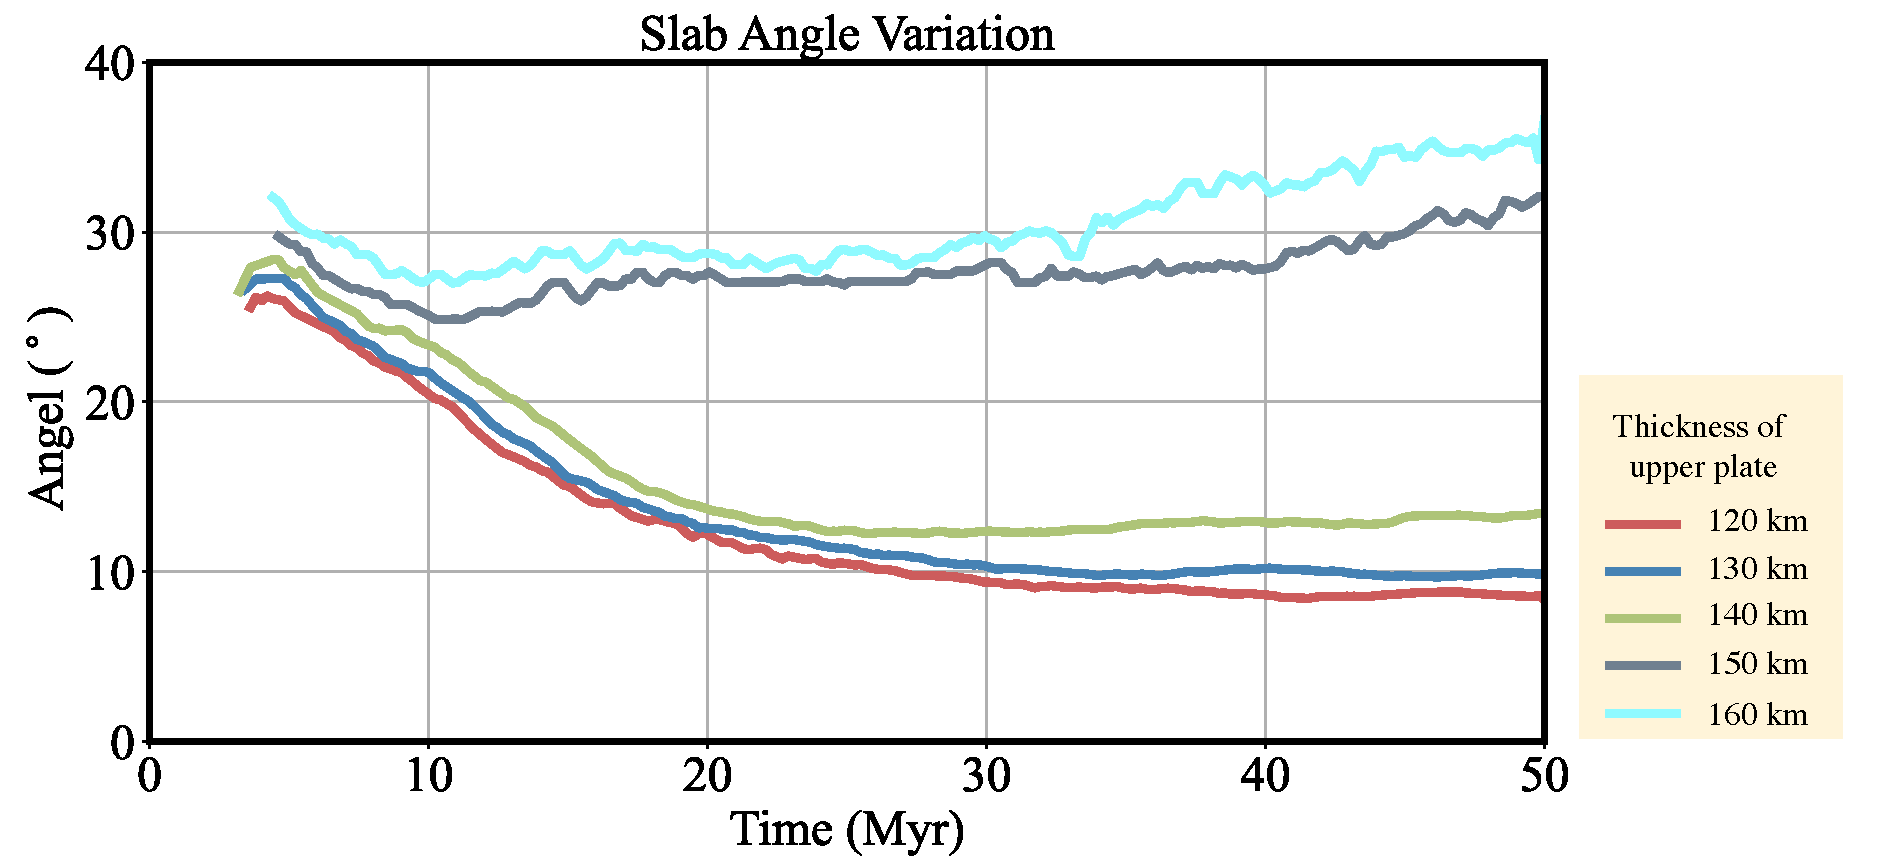
\includegraphics[width=6in]{compare_dip_thermal_Nazca_v2.pdf}
    \caption[測試上覆板塊厚度模型之150公里以上隱沒傾角隨時間變化]{測試上覆板塊厚度模型之150公里以上隱沒傾角隨時間變化。}
    \label{fig::compare_dip_thermal}
\end{figure*}

該結果表明,上覆板塊厚度在140公里以內的隱沒傾角在模型時間20 Myr後可低於15$^\circ$以內,反之,上覆板塊厚度150公里與160公里的模型隱沒傾角在任何時間上都高於25$^\circ$。
若將每個模型的隱沒板塊頂部在相同模型時間內隨深度繪出,可獲得圖\ref{fig::compare_geometry}。
從圖中可見,平坦隱沒特徵僅出現在上覆板塊厚度為120公里、130公里、140公里的三個模型中,而上覆板塊厚度150公里與160公里的兩個模型則是正常傾角的隱沒帶。
這意味著上覆板塊的溫度構造會大程度的影響隱沒板塊的隱沒構造,並且,高溫的環境較容易生成平坦隱沒。
此外,圖\ref{fig::compare_geometry}顯示平坦隱沒的平坦長度與深度在不同模型中有出入,藉由計算模型中平坦段的長度與深度,可獲得圖\ref{fig::compare_slab_time}

\begin{figure*}[ht!]
    \centering
    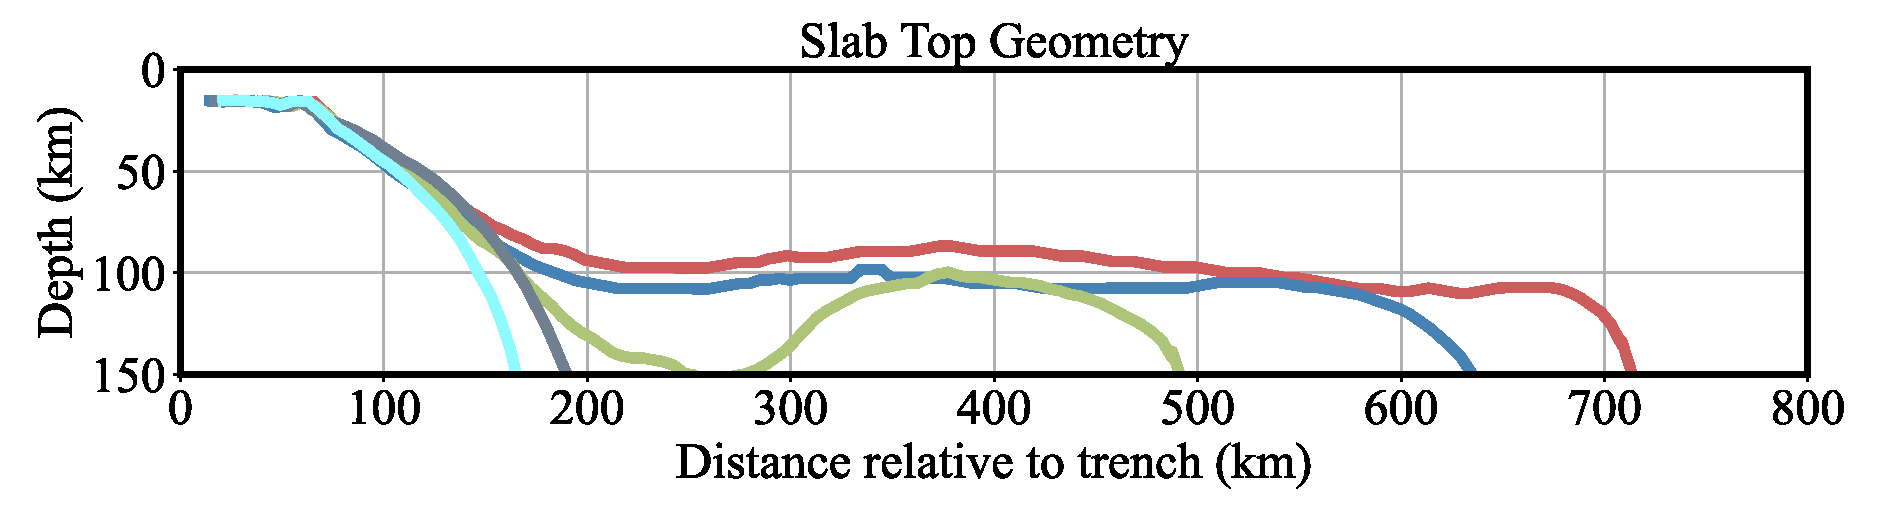
\includegraphics[width=6in]{slab_geometry_thermal_Nazca_v2.pdf}
    \caption[測試上覆板塊厚度模型在40 Myr的隱沒板塊構造]{測試上覆板塊厚度模型在40 Myr時隱沒板塊於150公里以上之構造,幾何形狀取自隱沒板塊頂部,使用5公里移動平均平滑離散化的網格,模型與圖\ref{fig::compare_dip_thermal}所使用的圖例相同。}
    \label{fig::compare_geometry}
\end{figure*}

較高溫的上覆板塊構造會在較淺的深度形成較長的平坦隱沒段,與\ref{智利參考模型結果}節的推測相同,平坦段深度大致與原先大陸岩石圈攝氏 800$^\circ$ 等溫線深度相同,因此較薄的大陸岩石圈有較淺的平坦隱沒段。
三個模型的平坦隱沒段長度差亦可達超過100公里。

\begin{figure*}[ht!]
    \centering
    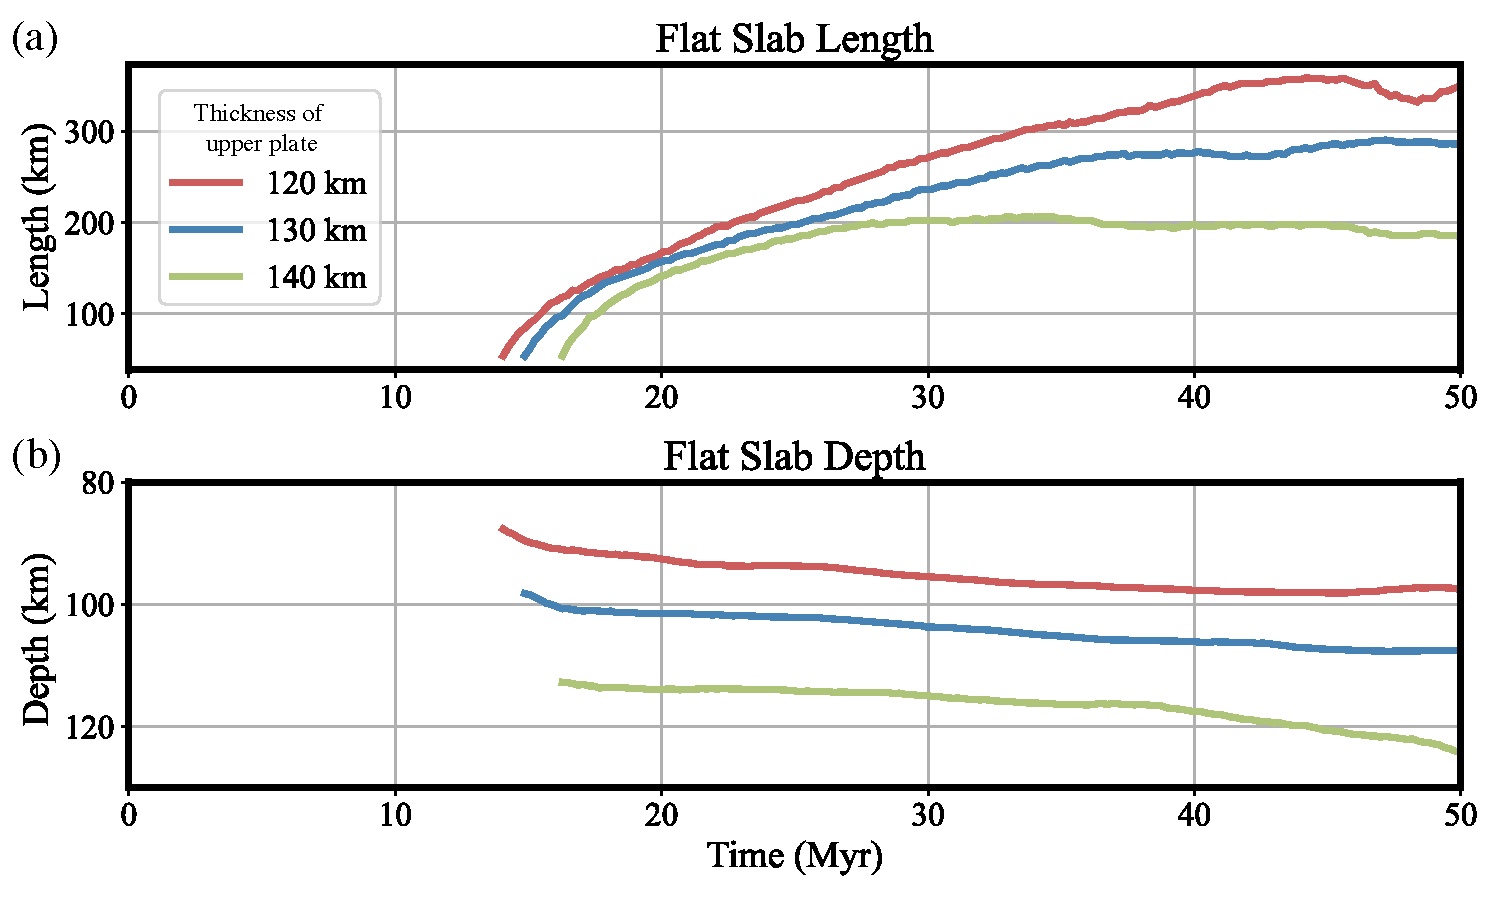
\includegraphics[width=5in]{thermal_Nazca_flatslab_length_v2.pdf}
    \caption[測試上覆板塊厚度模型的平坦段長度與深度]{測試上覆板塊厚度模型的平坦段(a)長度與(b)深度。模型與圖\ref{fig::compare_dip_thermal}所使用的圖例相同。}
    \label{fig::compare_slab_time}
\end{figure*}

這系列上覆板塊測試結果表明,較高溫的上覆板塊較容易形成平坦隱沒。
\citealp{liu2019influence}的數值模型利用改變上覆板塊的溫度構造與強度探討平坦隱沒的形成機制,他們的模型使用線性地溫梯度控制上覆板塊最終厚度,固定板塊底部的溫度為攝氏1336$^\circ$,並系統性測試模型中上覆板塊厚度自60-240公里對平坦隱沒的影響。
他們的結果顯示越薄、等深度下溫度越高的上覆板塊會形成深度越淺且長度越長的平坦隱沒段。
儘管他們的研究中,上覆板塊的溫度並不是決定平坦隱沒形成的關鍵因素,然而他們支持較高溫的上覆板塊較容易形成平坦隱沒,這項研究結果與本系列模型相似。
本研究認為,較高溫的大陸岩石圈具有黏滯度較低的岩石流變行為,因此岩石圈強度較低。
冷硬的隱沒板塊可能在大陸岩石圈強度較低的情況下輕易將岩石圈底部推開,形成長度較長的平坦隱沒段。

%他們的模型中,他們的結論表明較薄的上覆板塊比起冷硬的板塊更容易形成平坦隱沒,他們將結果歸因於較熱的上覆板塊具有黏滯度較小的地函岩石圈,進而導致隱沒板塊沿著
%容易促使平坦隱沒行成。

\subsubsection{墨西哥平坦隱沒的上覆板塊}
在墨西哥區域,\citealp{Manea2011Curie}曾經利用地磁資料計算墨西哥南部的居禮溫度(Curie temperature)面深度,進而獲得隱沒帶區域的溫度構造觀測資料。
在他們的研究中,針對兩條垂直於海溝的剖面進行討論,一條剖面為平坦隱沒段,另一條剖面為正常隱沒段。

平坦隱沒剖面在弧後區域具有較淺的居禮溫度面,由地磁獲得的估計居禮溫度面在弧後區深度約20-25公里,由他們研究中的熱模型推得的居禮溫度面深度約30公里左右,本研究墨西哥參考模型初始穩定大陸的居禮溫度面深度為28.5公里。

正常隱沒剖面的居禮溫度面範圍較大,地磁資料的結果落在15-30公里不等,不過他們的熱模型結果表示居禮溫度面在弧後區約落在42公里左右(見圖\ref{fig::Curie_Point_model})。
比較\citealp{Manea2011Curie}中的熱模型與本研究模型結果,測試一組居禮溫度面為38公里的初始墨西哥模型。
該模型在40公里前淺部地溫梯度為每公里攝氏15$^\circ$,而參考模型的地溫梯度為每公里攝氏20$^\circ$。

\begin{figure*}[ht!]
    \centering
    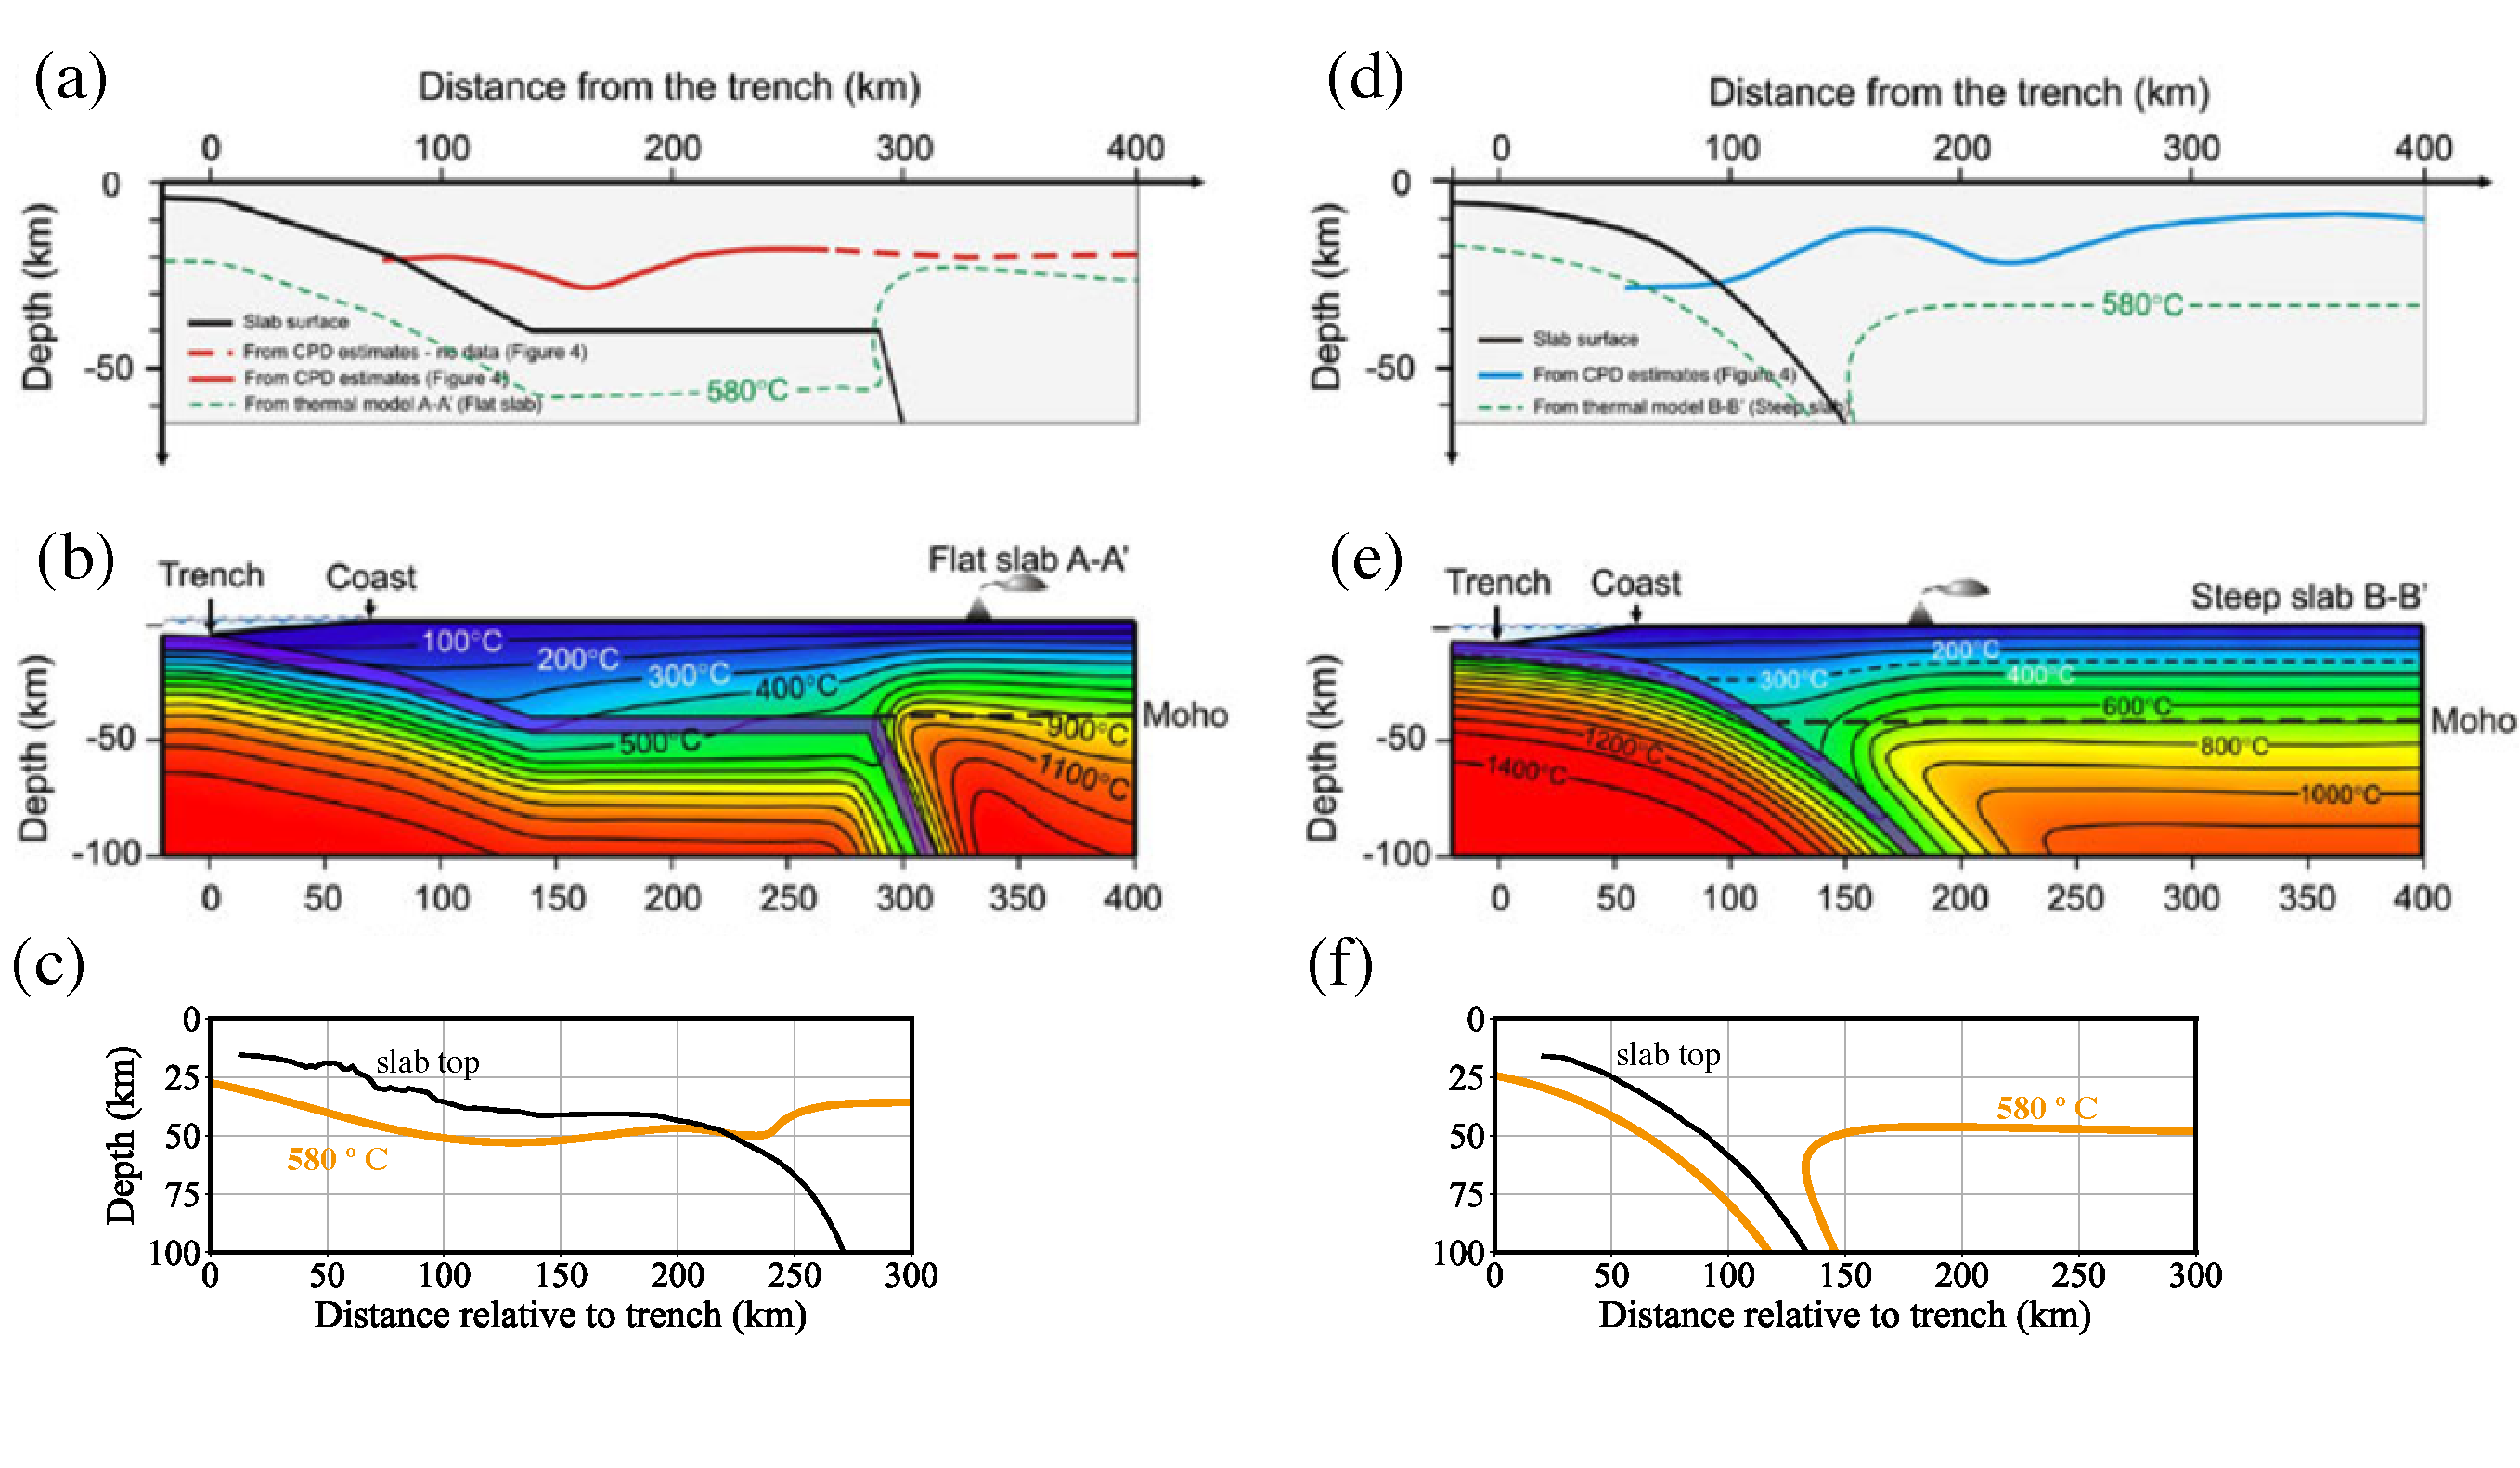
\includegraphics[width=6in]{CurieMexico_v3.pdf}
    \caption[墨西哥兩條剖面的居禮溫度面與熱構造模型與不同地溫梯度的墨西哥模型在30 Myr的隱沒板塊構造與580$^\circ$等溫線]{(a)(b)(d)(e)墨西哥兩條剖面的居禮溫度面與熱構造模型,摘自\citealp{Manea2011Curie}。(c)(f)不同地溫梯度的墨西哥模型在30 Myr的隱沒板塊構造(黑線)於100公里以上之剖面與580$^\circ$等溫線(橘線),幾何形狀取自隱沒板塊頂部,使用5公里移動平均平滑離散化的網格。(a)繪出平坦隱沒區域的居禮溫度面(紅線,虛線為外差值)、隱沒板塊頂部(黑線)與\citealp{Manea2011Curie}中熱模型攝氏580$^\circ$等溫線。(b)\citealp{Manea2011Curie}的平坦隱沒熱模型。(c)墨西哥參考模型在30 Myr的隱沒板塊構造(黑線)於100公里以上之剖面與580$^\circ$等溫線(橘線)。(d)繪出正常隱沒區域的居禮溫度面(藍線)、隱沒板塊頂部(黑線)與\citealp{Manea2011Curie}中熱模型攝氏580$^\circ$等溫線。(e)\citealp{Manea2011Curie}的正常隱沒熱模型。(f)測試一組於地表至40公里中每公里攝氏15$^\circ$的模型。模型於30 Myr的隱沒板塊構造(黑線)於100公里以上之剖面與580$^\circ$等溫線(橘線)。
    }
    \label{fig::Curie_Point_model}
\end{figure*}

圖\ref{fig::Curie_Point_model}顯示與\citealp{Manea2011Curie}類似的居禮溫度面結果,並且,與智利參考模型的結論相似,較高溫的大陸岩石圈較容易產生平坦隱沒。
本研究認為,儘管較高的岩石圈溫度會導致地函黏滯度降低,進而降低作用在隱沒板塊上的動水壓力,然而溫度升高同時導致岩石圈強度下降,此時隱沒板塊容易將弱的地函岩石圈推開,促使平坦隱沒發育。
不過該解釋屬於被動的平坦隱沒生成原因,本研究認為,墨西哥平坦隱沒是一極為年輕的海洋地殼隱沒,故重力力矩原先便小於其他隱沒帶區域,又加上

\newpage
\subsection{地函楔中的動水壓力力矩}
由於本研究中,只有智利參考模型的平坦隱沒上方包含地函楔,因此本節僅會測試與討論智利參考模型。
\citealp{Manea2007}與\citealp{Yan2020}提及隱沒帶脫水作用應是對動水壓力力矩有重大影響的因素之一。
大量的脫水會降低地函楔黏滯度與地函岩石強度,因此可能會降低地函動水壓力力矩的量值。
除了脫水作用外,岩漿作用也是另一個會影響地函楔黏滯度與岩石強度的因素(\citealp{jamieson2011crustal})。
在模型中,當地函楔發生部分熔融後,岩漿庫所產生的潛熱造成地函楔局部溫度增加,進而降低地函楔的黏滯度。
過去的數值模型鮮少討論岩漿作用對隱沒系統的動水壓力力矩影響,因此本研究對岩漿參數做一系列測試,用以探討兩者的關聯。
本節會先利用蛇紋岩厚度測試脫水作用對動水壓力力矩的影響,再討論岩漿作用與動水壓力力矩的關係。

\subsubsection{隱沒帶的脫水作用}
本研究數值模型的蛇紋岩產生量可自由控制(見\ref{蛇紋岩化的橄欖岩}節),本研究中,與普通橄欖岩相比,蛇紋岩具有較低的活化能(\citealp{hilairet2007high}),並約略等同於欖岩中有15$\%$之橄欖岩被蛇紋岩化。
模型中蛇紋岩的厚度可是為隱沒帶中脫水作用的活躍度,越厚的蛇紋岩可視為越劇烈的脫水環境。
因此本研究利用測試隱沒系統中不同蛇紋岩厚度探討脫水作用對智利參考模型的影響。
受限於網格解析度,因此測試厚度為2.5公里、5公里、7.5公里、10公里與15公里,每個模型的參數見表\ref{模型參數列表}b。
若將每個模型的隱沒板塊頂部在相同模型時間內隨深度繪出,可獲得圖\ref{fig::slab_geometry_serpentinite_thickness_Nazca_top}。

\begin{figure*}[ht!]
    \centering
    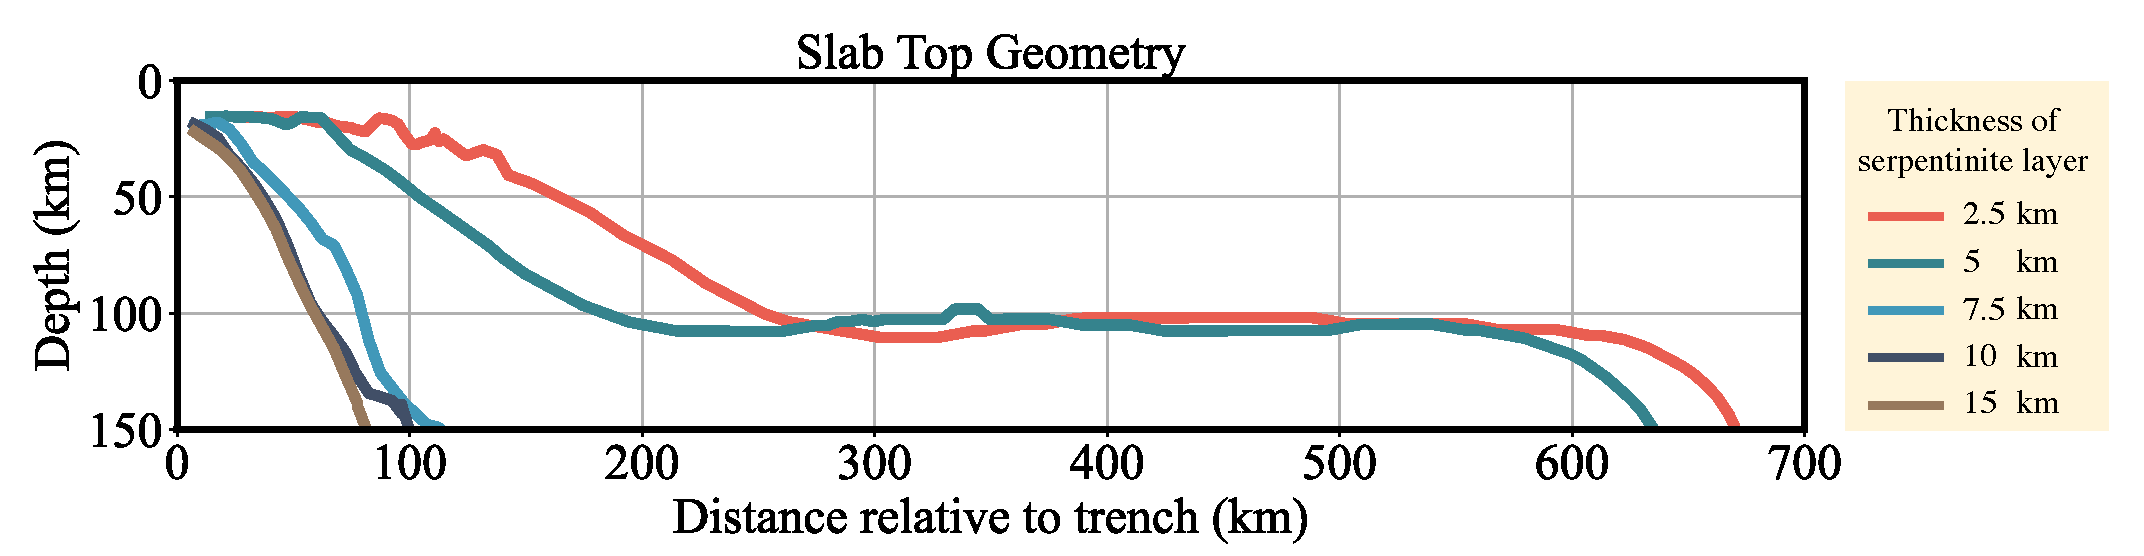
\includegraphics[width=5in]{slab_geometry_serpentinite_thickness_Nazca_v2.pdf}
    \caption[測試蛇紋岩厚度模型的隱沒板塊頂部剖面圖]{測試蛇紋岩厚度模型的隱沒板塊頂部剖面圖,使用5公里移動平均平滑離散化的網格。}
    \label{fig::slab_geometry_serpentinite_thickness_Nazca_top}
\end{figure*}

結果表明,只有蛇紋岩厚度為2.5公里與5公里的模型為平坦隱沒,亦即較活躍的脫水作用不容易形成平坦隱沒。
本系列模型之動水壓力力矩隨時間變化圖(圖\ref{fig::serpentinite_thickness_Nazca_suction})可見兩者的動水壓力力矩於10 Myr後開始呈現兩極化,蛇紋岩厚度為2.5公里與5公里的模型動水壓力力矩在10 Myr後快速增加。
從圖\ref{fig::serpentinite_thickness_Nazca_compare_viscosity}c來看,地函楔中的低壓帶於10 Myr後形成,是動水壓力力矩的增加主因。
反觀蛇紋岩厚度超過5公里的模型,動水壓力力矩在10 Myr之後便趨近於0,因此模型無法形成平坦隱沒。
圖\ref{fig::serpentinite_thickness_Nazca_compare_viscosity}d中顯示蛇紋岩厚度為7.5公里的模型動水壓力剖面,儘管模型在10 Myr有地函楔低壓帶存在,然而於12 Myr前後地函楔壓力明顯高於蛇紋岩厚度5公里的模型(圖\ref{fig::serpentinite_thickness_Nazca_compare_viscosity}c),隨後至14 Myr,地函楔低壓帶已逐漸與周遭地函平衡。
圖\ref{fig::serpentinite_thickness_Nazca_compare_viscosity}b是蛇紋岩厚度為7.5公里的模型的黏滯度剖面,可見軟流圈在12 Myr後進入原先地函楔低壓區,此時,隱沒板塊上下的壓力差趨近於0,動水壓力力矩降低。

\begin{figure*}[ht!]
    \centering
    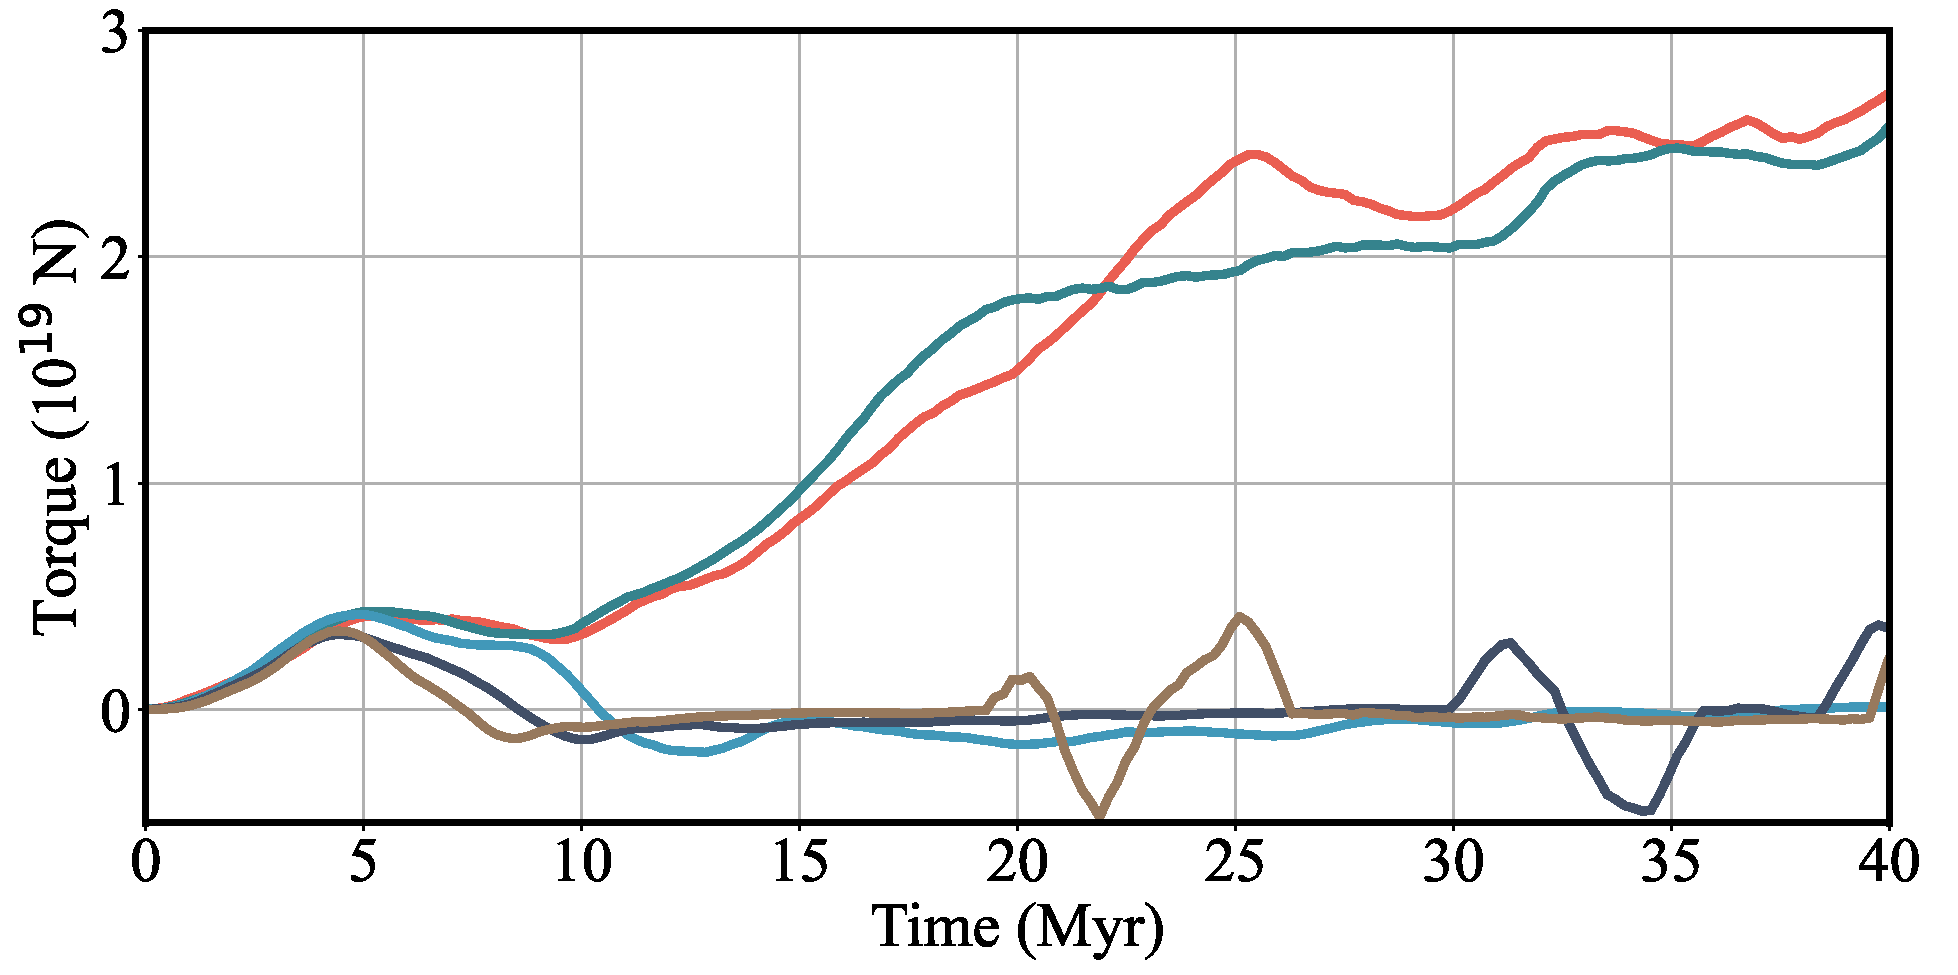
\includegraphics[width=5in]{serpentinite_thickness_Nazca_suction_v1.pdf}
    \caption[測試蛇紋岩厚度模型之動水壓力力矩]{測試蛇紋岩厚度模型之動水壓力力矩,模型與圖\ref{fig::slab_geometry_serpentinite_thickness_Nazca_top}所使用的圖例相同。}
    \label{fig::serpentinite_thickness_Nazca_suction}
\end{figure*}
從模型中的黏滯度剖面圖\ref{fig::serpentinite_thickness_Nazca_compare_viscosity}可見板塊交界處有一細窄低黏滯度通道,假設低黏滯度通道的寬度為隱沒板塊與上覆板塊之間黏滯度低於10$^{21}$ Pa$\cdot$s的寬度。
兩個模型間的低黏滯度通道在模型時間10 Myr表現出可辨別的寬度差,在這裡為蛇紋岩厚度的影響。
相對於地函岩石圈中的低壓環境,地函岩石圈中的軟流圈動水壓力較大,較厚的低黏滯度通道導致溫暖的軟流圈容易藉由壓力差流入板塊交界處中,
一旦低黏滯度通道與軟流圈相互連結,地函流容易流入地函岩石圈,導致隱沒板塊交界處形成一開放系統。
此時,地函岩石圈中原先的低壓環境隨著地函流的流入而消失,可見圖\ref{fig::serpentinite_thickness_Nazca_compare_viscosity}中10-14 Myr間動水壓力的變化。

\begin{figure*}[htp!]
    \centering
    \includegraphics[width=6in]{serpentinite_compare_Nazca_v1.pdf}
    \caption[測試蛇紋岩厚度模型於5 Myr、10 Myr、12 Myr與14 Myr之黏滯度與動水壓力剖面]{測試蛇紋岩厚度模型於5 Myr、10 Myr、12 Myr與14 Myr之黏滯度與動水壓力剖面。(a)蛇紋岩厚度為5公里的模型黏滯度剖面。(b)蛇紋岩厚度為7.5公里的模型黏滯度剖面。(c)蛇紋岩厚度為5公里的模型動水壓力剖面。(d)蛇紋岩厚度為7.5公里的模型動水壓力剖面。}
    \label{fig::serpentinite_thickness_Nazca_compare_viscosity}
\end{figure*}

\newpage
\subsubsection{隱沒帶的岩漿作用}
本研究數值模型岩漿作用與多個參數有關,控制著岩漿庫的增加速率與冷卻速率,詳細方法可見\ref{岩漿作用}節。
為了瞭解岩漿作用對隱沒系統的影響,本研究測試岩漿產生速率P$_0$與岩漿冷卻衰變常數$\lambda_0$分別為P$_k$與$\lambda_k$的倍數,獲得共12個模型,其中P$_k$=4.5$\times$10$^{-13}$,$\lambda_k$=1.6$\times$10$^{-12}$。
詳細的模型參數可見表\ref{模型參數列表}與圖\ref{fig::magma parameter}。

\begin{figure*}[ht]
    \centering
    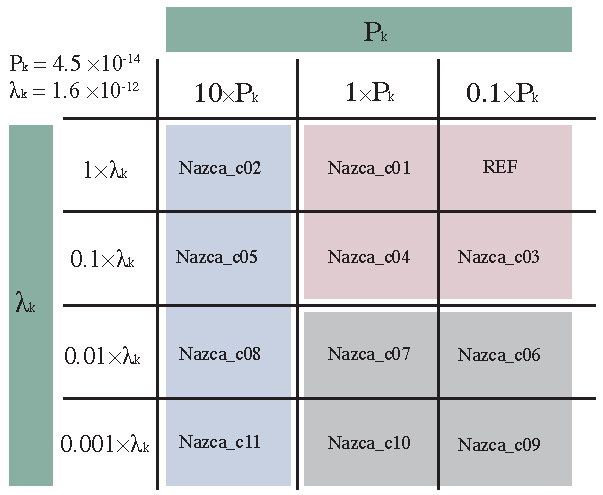
\includegraphics[width=4in]{magma parameter.pdf}
    \caption[智利模型岩漿參數測試示意圖,詳細岩漿參數見表\ref{模型參數列表}]{智利模型岩漿參數測試示意圖,詳細岩漿參數見表\ref{模型參數列表}。底部顏色為圖\ref{fig::magma_area_compare_Nazca}中的說明顏色。}
    \label{fig::magma parameter}
\end{figure*}

這系列模型結果顯示兩極化的隱沒板塊幾何狀態,可分為具有平坦隱沒的模型與正常隱沒模型。
若將每個模型的隱沒板塊頂部隨深度繪出,可獲得圖\ref{fig::magma_area_compare_Nazca}a。
圖中藍線則為此系列模型中正常隱沒模型的隱沒板塊頂部,隱沒板塊的幾何曲線幾何形狀趨近於一致。
紅線與黑線為此系列模型中具有平坦隱沒特徵的隱沒板塊頂部,平坦隱沒的深度並沒有明顯變化,不過隱沒板塊的曲線又可約略被分為兩群。
紅線群為平坦段斜率變化較小的一群模型,反之為黑線群。
紅線群包含岩漿冷卻衰變常數$\lambda_0=1.6\times 10^{-12}$與$\lambda_0=1.6\times 10^{-13}$,而黑線包含岩漿冷卻衰變常數$\lambda_0=1.6\times 10^{-14}$與$\lambda_0=1.6\times 10^{-15}$。
該結果可能可以為平坦隱沒在部分區域有強烈曲率變化提供一可能的影響原因。
秘魯區域的平坦隱沒南段具有劇烈的斜率變化(見圖\ref{fig::Peru_tomography}),\citealp{Ma2015}的接收函數研究發現該劇烈曲率變化與莫荷面深度平行,因此他們認為可能是地函岩石圈中強烈的動水壓力對隱沒板塊造成影響。
智利平坦隱沒板塊在平坦段並沒如此劇烈的斜率變化。

在這組參數測試中,岩漿產生速率很大程度上影響岩漿庫的體積大小,岩漿產生速率(P$_0$)越大,則岩漿庫的體積越大。
而岩漿冷卻衰變參數則控制岩漿庫生成後體積量的維持時間,岩漿冷卻參數越大,則岩漿冷卻速度越快,岩漿庫體積越快減少。
岩漿庫體積量隨時間變化之結果如圖\ref{fig::magma_area_compare_Nazca}b。

\begin{figure*}[ht!]
    \centering
    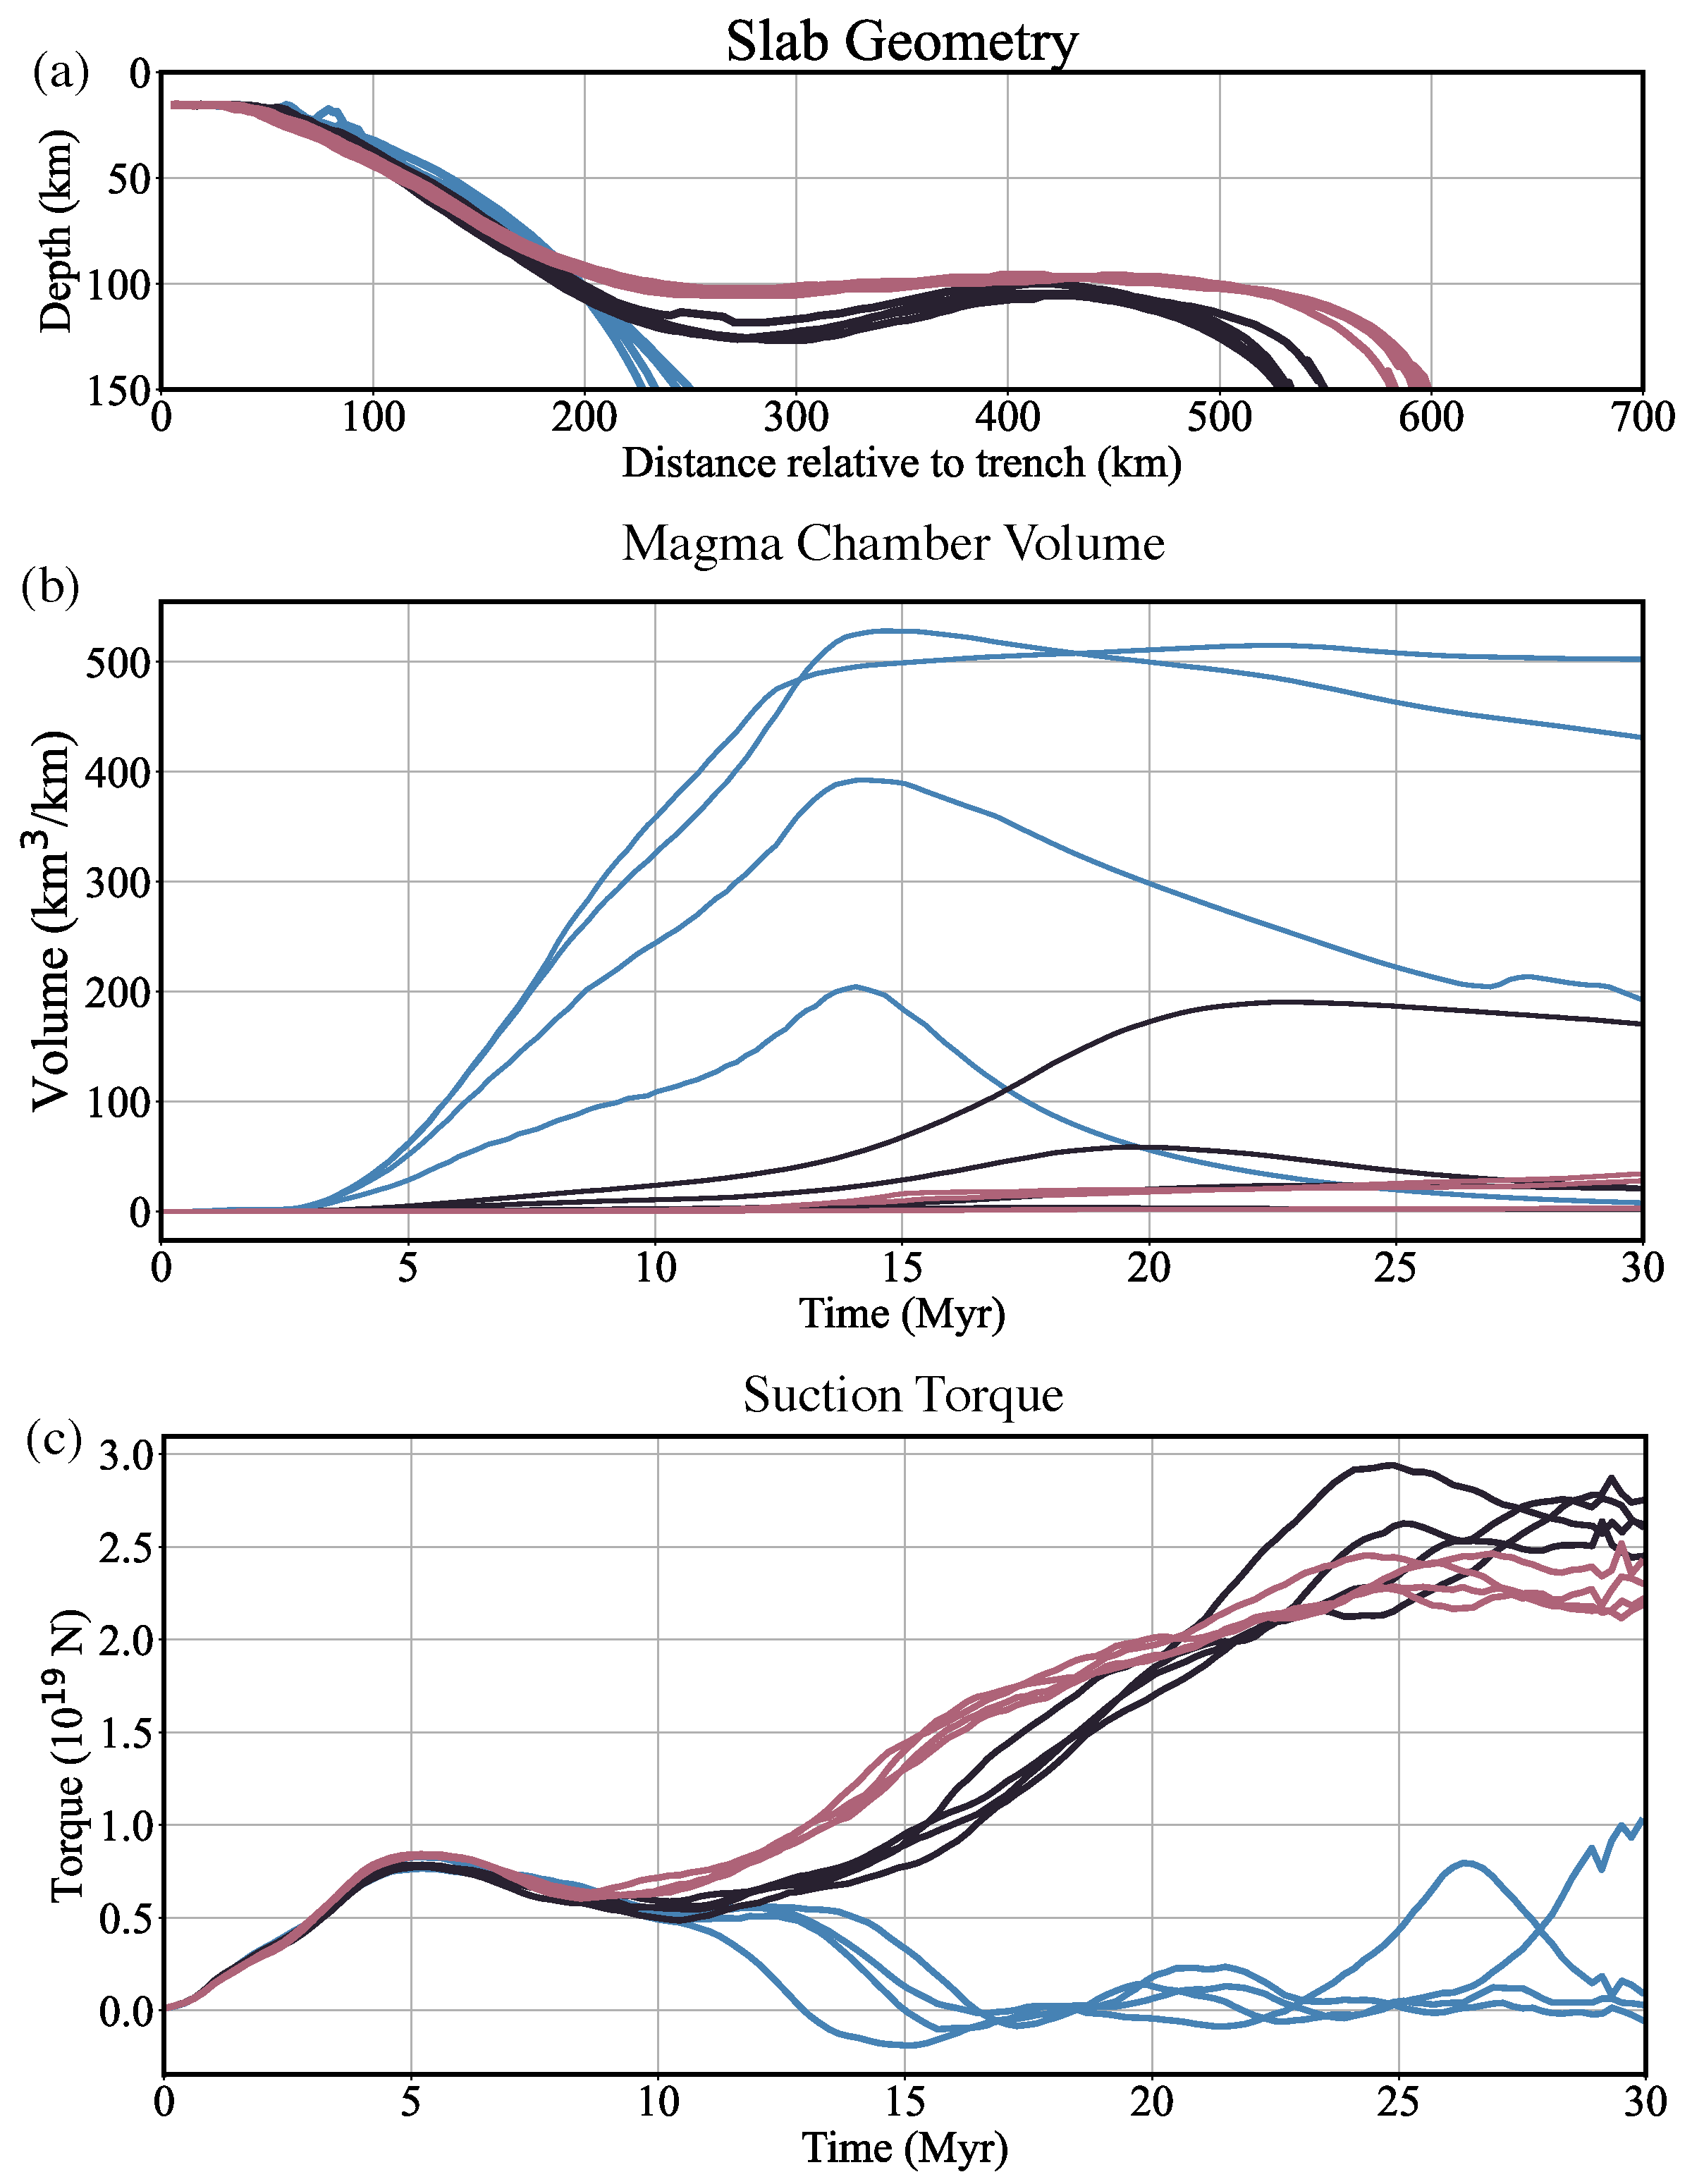
\includegraphics[width=5in]{magma_area_compare.pdf}
    \caption[智利模型岩漿參數測試結果,詳細岩漿參數見表\ref{模型參數列表}與圖\ref{fig::magma parameter}]{智利模型岩漿參數測試結果,詳細岩漿參數見表\ref{模型參數列表}與圖\ref{fig::magma parameter}。圖中不同線條(模型間)的顏色分類與圖\ref{fig::magma parameter}相同,共將模型分成三群。(a)隱沒板塊幾何形狀。(b)所有模型岩漿庫體積隨時間變化。(c)所有模型動水壓力力矩隨時間變化。}
    \label{fig::magma_area_compare_Nazca}
\end{figure*}

這些模型中,當岩漿產生速率為10 P$_k$ (P$_0$ =4.5$\times$10$^{-13}$)時,岩漿庫體積在5 Myr後開始顯著增加,並且在15 Myr前岩漿庫體積達到最高峰。
一旦模型中的岩漿庫在15 Myr年之前體積超過200 km$^3$/km,則模型變會成為一正常隱沒帶,而非平坦隱沒。
因此岩漿庫的體積可能會影響地函中的動水壓力力矩。
動水壓力力矩隨時間變化結果如圖\ref{fig::magma_area_compare_Nazca}c,動水壓力力矩在15 Myr前後呈現兩極化,在岩漿產生速率P$_0$=4.5$\times$10$^{-13}$的模型中,動水壓力力矩皆快速下降。

岩漿於冷卻過程中會釋放潛熱,導致地函楔中溫度升高。
而由於溫度與黏滯度有高度相關性,因此,越大量的岩漿體積會導致地函溫度較高,進而降低地函黏滯度,
與脫水作用的影響相同,地函岩石圈中若具有較低的黏滯度,容易促成溫暖的軟流圈與地函楔相連結,
又因為相對於地函楔中原先的低壓環境,軟流圈動水壓力較高,因此一旦岩石黏制度夠低,軟流圈地函流可輕易上湧進入板塊交界處中。
地函流流入地函岩石圈後,地函楔的低壓環境逐漸消失,因此施加於隱沒板塊上的動水壓力矩變低,隱沒系統不容易形成平坦隱沒。

這系列模型中可初步說明,岩漿作用有可能會大程度地減少隱沒帶的動水壓力,與隱沒帶脫水作用所扮演的角色相同。
早期地函動力學中計算隱沒系統之解析解,認為作用在隱沒板塊上的吸力極大,因此判斷地球早期大部分的隱沒系統皆為平坦隱沒(\citealp{tovish1978mantle}; \citealp{vlaar1983thermal}; \citealp{abbott1994flat})。
隨著地震站的廣設,現今全球隱沒板塊模型(\citealp{hayes2018slab2})顯示平坦隱沒並不常見於現今隱沒帶。
近年來數值模型表明地函吸力在早期被低估,隱沒板塊的脫水與地函楔的水合作用會產生低黏滯度地函楔,大幅降低地函吸力,因此真實的地函吸力應遠低於過去認知(\citealp{Manea2007})。
地函的動水壓力與地函中的溫度、壓力、岩石強度等性質有關,除了脫水作用外,本研究認為岩漿作用可能是另一個影響地函動水壓力的主要作用。


%\section{本研究的不足之處}
%
%1. 近年來的研究支持平坦隱沒可能與隱沒板塊與660不連續面的交互作用有關(\citealp{chen2019southward}; \citealp{schellart2020control}; \citealp{Schellart2021}),然而本研究智利參考模型僅300公里,無法參與這部分的討論。

%2. 在智利參考模型中,平坦隱沒的特徵在隱沒早期便出現,亦即該模型並不是從一正常傾角的隱沒帶漸變成平坦隱沒。
%納茲卡隱沒帶的已存在超過150 Ma,諸多研究表明(\citealp),平坦隱沒的發育時間約從10 Myr前後開始,在更早期的隱沒板塊應為正常傾角。


%本研究的墨西哥模型平坦段長度隨時間逐漸變長,只包含該區域平坦隱沒演化的前半段。
%本研究目前只能提供影響動水壓力的因素,但無法量化其影響動水壓力的量值。


% 參考文獻
% References
\refmatter
\bibliographystyle{abbrv}
\bibliography{back/references}

% 附錄
% Appendices
% !TeX root = ../main.tex

\appendix{A}{Introduction}
\section{Introduction}
\section{Further Introduction}

% !TeX root = ../main.tex

\appendix{B}{Introduction}
\section{Introduction}
\section{Further Introduction}


\end{document}
